\documentclass[letterpaper, 12pt]{article}
\usepackage[utf8]{inputenc}
\usepackage[spanish]{babel}
\usepackage[T1]{fontenc}
\usepackage{graphicx}
%\usepackage{comment}
%\usepackage{natbib}
%\usepackage{apacite}
%\usepackage[backend=biber,style=apa]{biblatex}
\usepackage{amssymb,amsmath,amsthm}
%\usepackage{subfigure} %incluir mas imagenes por figura
\usepackage{float}
\usepackage{verbatim}
\usepackage{fancyhdr}
\usepackage{setspace} % paquete para interlineado 
\usepackage{amssymb, amsmath, amsthm}
%\usepackage{appendix}
%\renewcommand{\appendixname}{Anexos}
%\renewcommand{\appendixtocname}{Anexos}
%\renewcommand{\appendixpagename}{Anexos}
\usepackage{pdfpages}

\usepackage{cite}
\usepackage[Algoritmo]{algorithm}
\usepackage{algorithmic}
%%\usepackage{textcomp}
\usepackage{xcolor}
\usepackage{array}

%agregadas independiente de la plantilla
\usepackage{soul}
\usepackage{subfig}
\usepackage{threeparttable}


\newlength\myindent
\setlength\myindent{2em}
\newcommand\bindent{%
  \begingroup
  \setlength{\itemindent}{\myindent}
  \addtolength{\algorithmicindent}{\myindent}
}
\newcommand\eindent{\endgroup}


\sloppy
%\pagestyle{fancy}
\renewcommand{\sectionmark}[1]{\markright{#1}{}}
\rhead{\large\thepage}  %  right header: document title
\lhead{\small\bfseries \nouppercase{\leftmark}}
\cfoot{}

%\geometry{left=3cm, right=2.5cm, top=3cm, bottom=3cm}
\newtheorem{teo}{{\sc Teorema}}

\pretolerance=3000
\tolerance=3000
\oddsidemargin 1.0cm \headsep 0.5cm \textwidth=15.5cm \textheight=22cm
\usepackage{pgfplots}
\usetikzlibrary{patterns}
\pgfplotsset{compat=1.5, tick label style={font=\scriptsize}, label style={font=\scriptsize}, legend style={font=\scriptsize}}



\begin{document}
\newcommand{\etal}[0]{\textit{et al.}}
\renewcommand{\tablename}{Tabla}
\renewcommand{\listtablename}{{\'I}ndice de tablas}

%\maketitle
\setcounter{secnumdepth}{3}
\setcounter{tocdepth}{3}

\begin{center}
\vspace*{-6.8cm}
\vbox{
	\begin{flushleft}\centering
		{\large{\textbf{UNIVERSIDAD CAT\'OLICA DEL MAULE}}\\
			Facultad de Ciencias de la Ingenier\'ia\\
			Mag\'{i}ster en Ciencias de la Computaci\'{o}n}
\end{flushleft}}

\vspace{7cm}

\begin{figure}
	\centering
	
\includegraphics[width=0.5\linewidth]{fig/logo.png}
\end{figure}


\begin{center}
	\Large{
	\textbf{Generación de ECG sintéticos mediante un modelo paramétrico de gaussianas asimétricas}
	}
\end{center} 
\vspace{1cm}
\begin{center}
	\Large {\textbf{Sebastián Jehovany Cerpa Gutiérrez}}\\
	\vspace{1cm}

	
	    \begin{tabular}{rl}
	         Director: & Dr. Juan Luis López Díaz\\
	         Co-Director: & Dr. Nombre co-director1\\
	         Co-Director: &  Dr.Nombre co-director2\\
	    \end{tabular}

	   \vspace{0.5cm}
	\textmd{Tesis de grado presentada en conformidad a los requisitos para obtener el grado de Mag\'{i}ster en Ciencias de la Computaci\'{o}n}
	
	
	
	\vspace{3.2cm}
	{\large { Talca, Septiembre 2026}}
	
\end{center} 

\thispagestyle{empty} \vspace*{2.0cm} 
\end{center}
\newpage
\thispagestyle{empty}
%\vspace*{-3cm}
%\hspace{-3cm}
%\hbox{\vsize = 5 cm
%\vbox{\hsize = 11cm

\vspace*{-3cm}
\hspace{-3cm}
\hbox{\vsize = 5cm
\vbox{\hsize = 11cm
\begin{flushleft}
\end{flushleft}}}

\begin{center}
    {\small {\bf UNIVERSIDAD CAT\'OLICA DEL MAULE}}\\
    \small {\bf FACULTAD DE CIENCIAS DE LA INGENIER\'IA}\\
    \small {\bf MAG\'ISTER EN CIENCIAS DE LA COMPUTACI\'ON}

\end{center}
\vspace{0.8cm}

\begin{center}
{\small {\bf TESIS PARA OPTAR AL}}\\
\small {\bf GRADO DE MAG\'ISTER EN CIENCIAS DE LA COMPUTACI\'ON}
\end{center}

\vspace{0.8cm}

\begin{center}
    {\small {\bf  Titulo de la tesis}}\\

\

\small {\bf Nombre alumno}\\
\end{center}

\vspace{0.8cm}

\begin{tabular}{l@{\hspace{1cm}}c@{\hspace{3cm}}l@{\hspace{1cm}}l}
{\bf COMISI\'ON EXAMINADORA}&&{\bf FIRMA}&\\
&&&\\
Director &&&\\
Dr. Nombre director1&&&\\
Universidad Cat\'olica del Maule\\
\cline{2-3}
&&&\\

Co-Director &&&\\
Dr. Nombre co-director1&&&\\
Universidad Cat\'olica del Maule\\
\cline{2-3}
&&&\\

Co-Director &&&\\
Dr. Nombre co-director2&&&\\
Universidad de...\\
\cline{2-3}
&&&\\

Revisor interno &&&\\
Dr. nombre revisor interno&&&\\
Universidad Cat\'olica del Maule\\
\cline{2-3}
&&&\\


Revisor externo&&& \\
Dr. Nombre revisor externo&&&\\
Universidad de...\\
\cline{2-3}
&&&\\


&&&\\
NOTA FINAL EXAMEN &&& \\
\cline{2-3}
\end{tabular}
\vspace{.7cm}


\begin{center}
{\large {\sc Talca, Mes Año}}
\end{center}

\newpage
%\input{TapaLFDP.tex}
\newpage
\newpage

\pagenumbering{roman}
\newpage

\section*{Agradecimientos}
\begin{spacing}{1.5}

Agradecimientos personales

\newpage
Agradecimientos formales (recursos, instituciones, proyectos, becas)

\end{spacing}

\begin{flushright}
Nombre1 Nombre2 Apellido1 Apellido2
\end{flushright}
\begin{flushright}
Mes Año
\end{flushright}

\newpage
\newpage
\section*{Resumen}
\begin{spacing}{1.4}

El desarrollo de sistemas de diagnóstico asistido por computadora mediante Inteligencia Artificial (IA) enfrenta un desafío crítico en cardiología: la escasez de datos etiquetados de alta calidad y el desbalance de clases en patologías raras. Esta investigación propone el desarrollo de un generador paramétrico de señales electrocardiográficas (ECG) sintéticas basado en la superposición de funciones Gaussianas asimétricas. A diferencia de los modelos de aprendizaje profundo (como las GANs), que carecen de control fisiológico y sufren de alucinaciones, este enfoque permite una parametrización explícita de la morfología P-QRS-T.

Mediante algoritmos de optimización numérica (L-BFGS-B) y utilizando registros de la base de datos MIT-BIH como semilla, el modelo calibra amplitudes, posiciones temporales y el nivel de la línea base para reproducir la morfología de señales reales. La validación se realizó sobre 2.237 latidos sinusales normales del registro 100 de dicha base, extraídos en una ventana asimétrica de 750 ms que contiene el complejo P-QRS-T completo, obteniendo una correlación de Pearson media de 0,9969 (desviación estándar 0,0015) y un RMSE medio de 0,0779 (desviación estándar 0,0148) en unidades de señal normalizada, con un sesgo del residuo indistinguible de cero.

Esta versión del trabajo incorpora además una segunda dimensión, ausente en la anterior: la organización temporal de la secuencia de latidos. Al modelo morfológico se le acopla un módulo de ritmo que produce la serie de intervalos entre latidos por síntesis espectral, con su exponente de escalamiento como parámetro de entrada declarado. El acoplamiento es selectivo en el tiempo: el complejo QRS no se estira con la frecuencia cardíaca, mientras que las ondas P y T sí. La validación de ese módulo no descansa en la indistinguibilidad respecto de una serie real, que fue el criterio del estado del arte, sino en la medición de una propiedad declarada: sobre una cohorte de cincuenta sujetos sintéticos de veinticuatro horas, el exponente pedido se recupera con un error absoluto medio de 0,014, y el sesgo del estimador queda caracterizado en función del largo del registro.

Estas cifras corresponden a la segunda iteración del modelo. Una primera implementación de veinte parámetros alcanzó una correlación de 0,9647 y un RMSE de 0,3985, y el análisis de su error residual identificó dos defectos concretos: la saturación del límite superior de amplitud de la onda R y la ausencia de un término de línea base. La corrección de ambos redujo el RMSE en un 87,6\% y llevó el sesgo sistemático del residuo a cero. El diagnóstico del residuo, y no solo la métrica agregada, resultó ser el instrumento que permitió esa mejora.

Los resultados obtenidos confirman la viabilidad del enfoque paramétrico para reproducir la morfología del ciclo P-QRS-T en ritmo sinusal normal. La incorporación de un motor de reglas basado en estándares clínicos (Rijnbeek/AHA) para simular variabilidad demográfica y patologías específicas se plantea como la extensión inmediata del trabajo, y no forma parte del alcance validado en esta etapa.

\end{spacing}

\newpage
\section*{Abstract}
\begin{spacing}{1.4}


\vspace{0.5cm}

\noindent\textbf{Keywords:} Synthetic ECG, Gaussian Models, Numerical Optimization, Physiological Variability, Data Augmentation.

\end{spacing}

\newpage

\thispagestyle{empty}
\tableofcontents
%\newpage\renewcommand{\listfigurename}{Índice de Figuras}
\newpage

%Indices de tablas y figuras
\listoffigures
\newpage
%\newpage\renewcommand{\listtablename}{Índice de Tablas}
\listoftables
\newpage
\pagestyle{fancy}
\newpage
\pagenumbering{arabic}


\newpage
%\chapter*{Introducción}

\section{Introducción}
\begin{spacing}{1.5}
\addcontentsline{toc}{section}{Introducción}
\markright{\MakeUppercase{Introducción}}

El avance exponencial de la Inteligencia Artificial (IA) en el sector salud ha inaugurado nuevas posibilidades para el diagnóstico asistido por computadora, prometiendo una detección más temprana y precisa de enfermedades cardiovasculares. Sin embargo, el desarrollo de modelos de IA robustos y fiables enfrenta un desafío estructural crítico: la dependencia de grandes volúmenes de datos de entrenamiento de alta calidad, diversos y correctamente etiquetados.

\subsection{Planteamiento del problema}

En el ámbito clínico, la conformación de estos conjuntos de datos es intrínsecamente compleja. Existen barreras significativas relacionadas con las estrictas normativas de privacidad del paciente, los elevados costos asociados al etiquetado manual por especialistas y, notablemente, la escasez y desbalance de clases. Este último punto es crítico: es difícil obtener registros suficientes de patologías raras o de grupos demográficos específicos, como neonatos o adultos mayores, lo que limita severamente la capacidad de generalización y la equidad de los sistemas de diagnóstico automático actuales.

Frente a esta problemática, esta investigación presenta el desarrollo de un modelo computacional generativo basado en la superposición de funciones Gaussianas asimétricas. Esta metodología se propone como una solución controlada y eficiente para la creación de señales sintéticas de electrocardiograma (ECG), permitiendo la aumentación de datos (data augmentation) con estricto apego a la morfología fisiológica y a las variaciones clínicas esperadas.

Para el desarrollo de esta investigación, se definen los siguientes conceptos rectores:

\textbf{Generación de Datos Sintéticos:} Proceso computacional mediante el cual se crean datos artificiales que imitan las propiedades estadísticas y estructurales de los datos reales. Su objetivo principal es enriquecer los conjuntos de entrenamiento, permitiendo que los algoritmos de aprendizaje automático aprendan patrones complejos sin comprometer la privacidad de pacientes reales ni depender exclusivamente de la recolección física de datos.

\textbf{Modelado Fenomenológico Paramétrico:} Enfoque matemático que describe la morfología de una señal biológica mediante la suma de funciones matemáticas predefinidas, priorizando la reproducción de la forma de la onda sobre la simulación de los procesos celulares subyacentes. En este estudio, se utiliza una combinación lineal de funciones Gaussianas para representar las ondas P, Q, R, S y T. Cada componente es controlada por parámetros optimizables de amplitud, posición temporal y ancho, lo que otorga una flexibilidad total para simular tanto la fisiología normal como variaciones patológicas específicas.

La relevancia de esta investigación radica en la urgencia de validar métodos alternativos y eficientes para la obtención de datos médicos para investigación. La capacidad de generar señales sintéticas de alta fidelidad, bajo demanda y a bajo costo, tiene el potencial de acelerar drásticamente el entrenamiento y validación de nuevas herramientas diagnósticas.

La pertinencia de utilizar un enfoque paramétrico basado en Gaussianas se fundamenta en la garantía de interpretabilidad y control fisiológico. Al construir la señal mediante parámetros matemáticos explícitos, el enfoque está diseñado para que los datos sintéticos no solo sean visualmente realistas, sino que respeten las reglas demográficas y clínicas establecidas (como la dependencia del intervalo QT respecto al sexo, o el ancho del complejo QRS respecto a la edad). Esto evita la generación de artefactos biológicamente imposibles, un requisito crucial para entrenar sistemas de IA que deban ser seguros, explicables y efectivos en un contexto clínico real.

\subsection{La dimensión que falta: el tiempo entre latidos}

El modelado morfológico descrito anteriormente resuelve la estructura individual del latido, pero omite una dimensión fisiológica fundamental: la dinámica temporal entre latidos sucesivos. Un generador que produce latidos morfológicamente correctos pero los emite a intervalos constantes, o con una variabilidad sin estructura, no produce un electrocardiograma: produce una secuencia de latidos. Y buena parte de la información que distingue un corazón sano de uno enfermo no reside en la forma de cada latido sino en la organización temporal de la serie que forman.

Peng et al.\ \cite{peng1995quantification} mostraron que el latido sano no se regula según el principio clásico de homeostasis, es decir reduciendo la variabilidad hacia un estado de equilibrio, sino que exhibe correlaciones de largo alcance propias de los sistemas dinámicos alejados del equilibrio; y que en insuficiencia cardíaca congestiva severa ese comportamiento correlacionado se degrada. En ese mismo trabajo introdujeron el análisis de fluctuaciones sin tendencia (DFA, por \emph{detrended fluctuation analysis}), que resume la estructura de correlación de una serie no estacionaria en un exponente de escalamiento α, y reportaron un cruce entre un exponente de corto alcance y otro de largo alcance.

Ese exponente dejó de ser una curiosidad matemática para convertirse en un descriptor con valores de referencia. Costa et al.\ \cite{costa2017fragmentation}, sobre registros de veinticuatro horas de 109 adultos sanos con edad mediana de 40 años, reportan un exponente de corto alcance $\alpha_1$ de $1{,}17$ (rango intercuartílico $1{,}07$--$1{,}27$), frente a $1{,}02$ ($0{,}81$--$1{,}15$) en pacientes con enfermedad coronaria. Las revisiones de métricas de variabilidad de la frecuencia cardíaca ubican a $\alpha_1$ y $\alpha_2$ entre los índices no lineales de uso corriente, calculan $\alpha_1$ sobre ventanas de menos de once latidos, y advierten que el DFA exige registros de varias horas \cite{shaffer2017overview,sundas2025hrv}.

Conviene enunciar con cuidado qué dice y qué no dice esa evidencia, porque la formulación intuitiva —orden en el enfermo, desorden en el sano— es a la vez sugerente y engañosa. Más variabilidad no es mejor: hay condiciones patológicas que la elevan, y en pacientes post-infarto un aumento de la variabilidad no lineal constituye un factor de riesgo independiente de mortalidad \cite{shaffer2017overview}. Lo que caracteriza a la salud no es un extremo sino un nivel óptimo; en palabras de esa misma revisión, un corazón sano no es un metrónomo, pero tampoco es ruido. La formulación defendible no es una dirección sino una degradación: la pérdida de las propiedades de escalamiento, que según la patología se manifiesta hacia valores más aleatorios o más regulares.

Frente a esa dimensión, los generadores existentes se reparten en dos familias que han permanecido notablemente separadas. Los generadores de forma de onda, cuyo referente es el modelo dinámico de McSharry et al.\ \cite{mcsharry2003dynamical}, eproducen la morfología del ciclo P-QRS-T pero gobiernan el ritmo con un espectro bimodal, construido como la suma de dos distribuciones gaussianas que representan la arritmia sinusal respiratoria y las ondas de Mayer, con la razón entre bandas de baja y alta frecuencia como parámetro de control. Un espectro así decae más rápido que cualquier ley de potencias fuera de sus picos, de modo que la serie generada no tiene estructura de largo alcance; en ese trabajo no aparece mención alguna a exponentes de escalamiento ni a comportamiento fractal.

La segunda familia genera la secuencia de intervalos y nada más. Su hito es el desafío PhysioNet/Computers in Cardiology de 2002 \cite{moody2002challenge}, que pidió a los participantes generar series sintéticas de intervalos R-R de veinticuatro horas y luego distinguirlas de las reales dentro de un conjunto sin etiquetar. El criterio de calidad fue, por lo tanto, la indistinguibilidad. Entre las entradas, McSharry et al.\ \cite{mcsharry2002tachogram} produjeron tacogramas de veinticuatro horas combinando el mismo espectro bimodal para el corto alcance con conmutaciones entre estados fisiológicos discretos —incluidos los estados de sueño—, cada uno con su propia media, varianza y tendencia extraídas de datos reales. Es decir: generar una serie de intervalos de veinticuatro horas es un problema resuelto desde 2002, y por los mismos autores del generador de forma de onda. Lo que ninguno de esos trabajos hace es tratar el exponente de escalamiento como un parámetro de entrada.

Para abordar esta dimensión, el presente modelo incorpora precisamente esa contribución. Al modelo morfológico se le agrega un módulo de ritmo que produce la serie de intervalos entre latidos por síntesis espectral, de manera que su exponente de escalamiento sea un parámetro que se declara y que después se verifica sobre la serie generada. Morfología y ritmo se acoplan de forma selectiva en el tiempo: el complejo QRS no se estira con la frecuencia cardíaca, porque su duración depende de la velocidad de conducción intraventricular, mientras que las ondas P y T sí lo hacen. Ese acoplamiento selectivo es sencillo en un modelo paramétrico, donde el centro y el ancho de cada onda son parámetros explícitos, y no lo es en un modelo de ecuaciones diferenciales, donde el ciclo completo se estira en bloque.

Una precisión de nomenclatura, porque en esta literatura es fuente permanente de error. El exponente de Hurst $H$ y el exponente $\alpha$ que entrega el DFA están relacionados pero no son intercambiables: para ruido gaussiano fraccional, que es estacionario, se cumple $\alpha = H$ con $\alpha$ entre 0 y 1; para movimiento browniano fraccional, que no lo es, se cumple $\alpha = H + 1$ con $\alpha$ entre 1 y 2 \cite{hardstone2012dfa}. Como los valores sanos de veinticuatro horas rondan $1{,}17$, es decir por encima de la unidad, caen fuera del rango que un generador de ruido gaussiano fraccional puede producir. Por esa razón este trabajo parametriza en $\alpha$ y no en $H$, y declara explícitamente el régimen supuesto cada vez que informa un valor de $H$.

\subsection{Hipótesis}

Es posible construir un generador de señales ECG sintéticas basado en la superposición de funciones Gaussianas y optimización numérica que reproduzca la morfología de señales reales con alta fidelidad estructural, permitiendo la parametrización controlada de variables distinguiendo entre sujetos sanos y enfermos.

Complementariamente, se plantea que es posible dotar a este generador de una dinámica latido a latido cuyo exponente de escalamiento sea un parámetro de entrada. Esta segunda proposición es verificable de manera independiente de la primera, y su verificación no descansa en la indistinguibilidad respecto de una serie real sino en la medición de una propiedad declarada.

\subsection{Objetivos}

\subsubsection{Objetivo general}

Diseñar un simulador computacional de señales de electrocardiograma basado en un modelo matemático paramétrico de Gaussianas asimétricas, capaz de generar conjuntos de datos sintéticos etiquetados para un grupo control de sujetos sanos y un grupo de sujetos enfermos.

\subsubsection{Objetivos específicos}

\begin{enumerate}

\item Implementar el modelo matemático de suma de Gaussianas asimétricas para la representación morfológica del ciclo cardíaco P-QRS-T.

\item Calibrar los parámetros del modelo mediante algoritmos de optimización (L-BFGS-B \cite{byrd1995limited} con restricciones de límites) utilizando latidos reales de la base de datos MIT-BIH Arrhythmia Database como ``semilla''.

\item Desarrollar un motor de reglas fisiológicas que adapte los parámetros de tiempo y voltaje según tablas de referencia clínica (Rijnbeek \cite{rijnbeek2001normal} y AHA \cite{rautaharju2009aha}) para simular pacientes sanos y enfermos.

\item Incorporar un módulo de ritmo que genere la secuencia de intervalos entre latidos con un exponente de escalamiento declarado como parámetro de entrada, acoplarlo al modelo morfológico de forma selectiva en el tiempo, y verificar la recuperación de ese exponente sobre las series generadas.

\item Validar la fidelidad de las señales generadas comparándolas con registros reales mediante métricas de correlación de Pearson, Error Cuadrático Medio (RMSE) y análisis en el dominio de la frecuencia.

\item Validar el conjunto de datos sintéticos mediante un modelo de red neuronal preentrenado.

\end{enumerate}

\subsection{Estructura del Trabajo}

El documento se organiza de la siguiente manera:

El Marco Teórico expone los fundamentos de la electrofisiología cardíaca y del modelado matemático de señales biomédicas necesarios para seguir el desarrollo posterior.

El Estado del Arte explora los antecedentes académicos en la generación de datos sintéticos biomédicos, contrastando los enfoques de modelado dinámico frente a los enfoques puramente estadísticos.

Los Métodos Propuestos describen el enfoque técnico implementado, detallando el diseño del modelo matemático de Gaussianas, el proceso de optimización numérica con datos reales (MIT-BIH), la integración de las reglas fisiológicas que distinguen sanos de enfermos y el módulo de ritmo parametrizado por el exponente de escalamiento.

Los Resultados Experimentales y Discusión presentan la validación estadística de las señales generadas sobre el registro 100 de la base MIT-BIH, el análisis del error residual y el contraste entre los objetivos proyectados y los efectivamente alcanzados.

Finalmente, las Conclusiones evalúan el cumplimiento de cada objetivo específico y delimitan las líneas de trabajo futuro.


\subsection{Alcance y delimitación del problema}

El alcance de esta investigación se delimita en los siguientes términos:

\textbf{Señales objeto de estudio.} El trabajo aborda la generación de latidos de electrocardiograma de superficie correspondientes a ritmo sinusal normal, en registros de una derivación. Se emplea el canal MLII de la MIT-BIH Arrhythmia Database \cite{moody2001impact}, y se procesan exclusivamente los latidos anotados como normales, descartando latidos ectópicos y segmentos con artefactos. Esos latidos constituyen la semilla morfológica del modelo. La condición de enfermo no se obtiene, por lo tanto, de latidos patológicos reales, sino del desvío controlado de los parámetros de tiempo y voltaje respecto de los rangos normales de referencia y de la dinámica del ritmo.

\textbf{Unidad de generación.} Se modelan dos unidades y su acoplamiento. La primera es el latido individual, segmentado en una ventana \emph{asimétrica} respecto del pico R: 250 ms antes y 500 ms después. La asimetría se sigue de la fisiología del complejo, dado que la onda P comienza cerca de 250 ms antes del pico R y la onda T termina entre 400 y 450 ms después, de modo que una ventana centrada no puede contenerlo. La segunda unidad es la secuencia de intervalos R-R, que en la versión anterior de este trabajo quedaba explícitamente fuera del alcance y que aquí se incorpora con su exponente de escalamiento como parámetro.

\textbf{Sobre el significado de las etiquetas.} Las etiquetas de sano y enfermo son etiquetas de construcción y no diagnósticos. Indican si los parámetros de tiempo y voltaje del sujeto sintético se generaron dentro o fuera de los rangos normales de referencia, y con qué exponente de escalamiento se generó su serie de intervalos. La precisión importa porque las distribuciones de $\alpha_1$ en poblaciones sanas y enfermas se solapan de manera sustancial \cite{costa2017fragmentation}, de modo que ningún valor particular del exponente identifica por sí solo una condición clínica. El generador declara cómo fue construido cada registro; no emite un diagnóstico sobre un paciente.

\textbf{Tamaño del conjunto generado.} Cada conjunto sintético se genera con 2.048 latidos, largo que permite estimar el exponente de escalamiento con holgura y alimentar el entrenamiento de un clasificador.

\textbf{Dimensión morfológica.} El modelo reproduce la morfología del ciclo P-QRS-T en amplitud y posición temporal. No aborda el ruido de línea base, la interferencia de red ni los artefactos de movimiento, que constituyen problemas de simulación distintos e independientes del modelado morfológico.

\textbf{Exclusiones explícitas.} Quedan fuera del alcance de esta etapa la generación multiderivación y la simulación de morfologías arrítmicas específicas, en particular la elevación del segmento ST mediante inyección de funciones de lesión y la Fibrilación Auricular mediante anulación de la onda P. Ambas figuraban como objetivo en la propuesta original y aquí se reclasifican como trabajo futuro, dado que la condición patológica se representa mediante desvíos de los parámetros de tiempo y voltaje y mediante la dinámica del ritmo, y no mediante morfologías ectópicas. Estas extensiones no constituyen resultados comprometidos.

Esta delimitación busca alinear el problema declarado con los objetivos específicos verificables, evitando que el alcance enunciado exceda a aquello que la validación experimental puede sustentar.

\end{spacing} 

\newpage
\section{Marco Teórico}\label{sec:background}
\begin{spacing}{1.5}

\subsection{Introducción}

Este capítulo establece los fundamentos necesarios para justificar las decisiones de modelado adoptadas en esta investigación. Se organiza en cuatro bloques: los fundamentos electrofisiológicos que dan origen a la señal electrocardiográfica, los paradigmas disponibles para modelarla matemáticamente, la justificación específica del uso de funciones Gaussianas, y la discusión sobre el papel del volumen de datos y de los enfoques supervisados y no supervisados en el diagnóstico asistido.

\subsection{Fundamentos electrofisiológicos de la señal electrocardiográfica}

El electrocardiograma es el registro en superficie corporal de la actividad eléctrica generada por la despolarización y repolarización sucesivas del miocardio. Su base celular fue establecida por Hodgkin y Huxley \cite{hodgkin1952quantitative}, quienes formularon una descripción cuantitativa del flujo de corriente iónica a través de la membrana mediante un sistema de ecuaciones diferenciales ordinarias que relaciona las conductancias de sodio y potasio con el potencial de membrana y el tiempo.

Noble \cite{noble1962modification} adaptó posteriormente dicho formalismo a las fibras de Purkinje cardíacas, cuyos potenciales de acción son de duración considerablemente mayor que los del axón de calamar originalmente estudiado, y en las que la despolarización disminuye la permeabilidad al potasio. Esta adaptación constituye el punto de partida del modelado biofísico del tejido cardíaco.

La evolución del campo desde la bioelectricidad celular hasta sus aplicaciones clínicas ha sido documentada bibliométricamente por Choca et al. \cite{choca2025electrofisiologia}, quienes reportan un crecimiento sostenido de la producción científica en electrofisiología cardíaca, con un incremento notable en las últimas dos décadas.

En el trazado de superficie, esta actividad se manifiesta como una secuencia característica de deflexiones: la onda P, correspondiente a la despolarización auricular; el complejo QRS, asociado a la despolarización ventricular; y la onda T, que refleja la repolarización ventricular. La interpretación sistemática de estas deflexiones y de los intervalos que las separan constituye una competencia clínica fundamental \cite{zumba2023evaluacion}.

Resulta relevante para esta investigación que la morfología considerada normal no es única. Corrado et al. \cite{corrado2009twelve} documentan que en atletas altamente entrenados la bradicardia sinusal alcanza prevalencias de hasta el 80\%, el bloqueo auriculoventricular de primer grado el 35\% y la repolarización temprana entre el 50\% y el 80\%, sin que ello constituya patología. La frontera entre variante fisiológica y hallazgo patológico depende del contexto demográfico del sujeto, lo que anticipa la necesidad de parametrizar dicho contexto en cualquier generador de señales sintéticas.

\subsection{Paradigmas de modelado de la señal electrocardiográfica}

La literatura ofrece tres familias de aproximaciones al modelado de señales ECG, que se distinguen por el nivel de descripción que adoptan.

\subsubsection{Modelos biofísicos}

Descienden directamente del formalismo de Hodgkin-Huxley \cite{hodgkin1952quantitative} y de su adaptación cardíaca \cite{noble1962modification}. Describen los mecanismos iónicos subyacentes y poseen, por tanto, el mayor poder explicativo. Su limitación para el propósito de esta investigación es doble: el costo computacional de integrar sistemas de ecuaciones diferenciales acopladas para cada latido, y el hecho de que su salida natural es el potencial de acción celular, no el trazado de superficie, cuya obtención requiere resolver adicionalmente el problema directo de la electrocardiografía.

\subsubsection{Modelos fenomenológicos dinámicos}

Renuncian a describir el mecanismo celular y se concentran en reproducir la forma de la onda. El referente del área es el modelo de McSharry et al. \cite{mcsharry2003dynamical}, que genera la señal mediante un sistema de tres ecuaciones diferenciales ordinarias acopladas cuya trayectoria recorre un ciclo límite tridimensional. El modelo reproduce con realismo la variabilidad de la frecuencia cardíaca y permite prescribir el espectro de potencia de los intervalos R-R.

Sus propios autores reconocen dos limitaciones pertinentes: la validación se apoyó en comparación visual sin reportar métricas cuantitativas de error, y los parámetros de los eventos P-QRS-T fueron derivados de análisis visual subjetivo.

\subsubsection{Modelos paramétricos por descomposición}

Describen la señal como una combinación lineal de funciones elementales cuyos parámetros se ajustan a datos reales. Clifford et al. \cite{clifford2004model} demostraron que la descomposición mediante suma de funciones Gaussianas es computacionalmente eficiente y permite una parametrización precisa de la asimetría de las ondas, propiedad especialmente relevante para representar morfologías isquémicas en las que el segmento ST resulta crítico.

\subsection{Justificación del uso de funciones Gaussianas}

La elección de la función Gaussiana como primitiva morfológica no es arbitraria, y conviene explicitar los cinco argumentos que la sostienen frente a las alternativas disponibles.

\textbf{Correspondencia con la forma de la señal.} Cada deflexión del ciclo P-QRS-T es un pulso unimodal, con un máximo bien definido y decaimiento a ambos lados. La Gaussiana es la función más simple que reproduce esa forma con únicamente tres parámetros, y presenta la ventaja de que cada uno posee interpretación fisiológica directa: la amplitud corresponde al voltaje de la deflexión, la posición al instante del evento eléctrico dentro del ciclo, y el ancho a su duración. Un ajuste de la onda R no produce coeficientes abstractos, sino magnitudes que un cardiólogo puede evaluar.

\textbf{Continuidad con el estándar del área.} El modelo de McSharry et al. \cite{mcsharry2003dynamical}, referente de la simulación de ECG, emplea internamente términos Gaussianos como forzamiento angular para generar la morfología P-QRS-T. Las Gaussianas ya son la primitiva morfológica del modelo dinámico de referencia. Adoptarlas directamente conserva esa base morfológica y elimina el costo de integrar el sistema de ecuaciones diferenciales, lo cual resulta determinante cuando el objetivo es generar volúmenes elevados de latidos.

\textbf{Ventaja frente a otras bases de descomposición.} Las bases ortogonales de propósito general, como las wavelets o los polinomios por tramos, permiten aproximar la señal con error arbitrariamente pequeño, pero sus coeficientes carecen de significado clínico: no existe un coeficiente wavelet que corresponda a la amplitud de la onda R. Dado que el propósito de esta investigación es generar señales con control fisiológico explícito, y no meramente comprimirlas o reconstruirlas, la interpretabilidad de los parámetros constituye un requisito y no una preferencia estética.

\textbf{Ventaja frente a los enfoques basados en redes neuronales informadas por la física.} Las Physics Informed Neural Networks constituyen una alternativa contemporánea para incorporar restricciones físicas al aprendizaje \cite{sophiya2025pinns}. Su aplicabilidad al problema abordado es limitada: requieren disponer de la ecuación diferencial que gobierna el fenómeno, y el ECG de superficie no admite una formulación compacta equivalente. La literatura reporta además dificultades de convergencia y un elevado costo computacional en problemas de alta dimensión.

\textbf{Extensión a la Gaussiana asimétrica.} La Gaussiana clásica es simétrica respecto de su centro, mientras que las deflexiones reales no lo son: la onda T presenta característicamente una fase ascendente más lenta que la descendente. Permitir anchos diferenciados a cada lado del centro captura esta propiedad al costo de un único parámetro adicional por onda, conservando la interpretabilidad del resto.

\subsection{El volumen de datos como limitante del diagnóstico asistido}

El desempeño de los modelos de clasificación automática de arritmias depende críticamente de la cantidad, la diversidad y la calidad de los datos anotados disponibles. Conviene precisar por qué este constituye un problema real y no un supuesto.

La MIT-BIH Arrhythmia Database \cite{moody2001impact} fue el primer conjunto estándar de acceso público y sigue siendo el referente de facto: reúne aproximadamente 110.000 anotaciones verificadas sobre 109.000 complejos QRS y ha sido empleada en cerca de 500 centros de investigación desde 1980. Su propia historia ilustra el costo del etiquetado: la anotación fue manual y verificada por cardiólogos, y 33 latidos distribuidos en 6 registros quedaron sin clasificar por desacuerdo entre especialistas. La etiqueta clínica no es un dato disponible sin costo, ni está exenta de ambigüedad.

A esta escasez se suma el desbalance de clases. Una base construida a partir de registros Holter refleja la prevalencia natural de cada condición, de modo que las patologías infrecuentes quedan representadas por un número reducido de ejemplos, precisamente aquellas cuya detección automática tendría mayor valor clínico.

La relevancia de este problema se aprecia en la epidemiología. Fox et al. \cite{fox2001coronary} determinaron que la enfermedad arterial coronaria fue la etiología del 52\% de los casos incidentes de insuficiencia cardíaca en población general, y que el 25\% de esos casos no había sido reconocido como coronario antes de la angiografía. El margen de mejora diagnóstica es sustantivo, y depende de herramientas entrenadas sobre datos suficientes.

Finalmente, la diversidad demográfica constituye una dimensión adicional del mismo problema. Rijnbeek et al. \cite{rijnbeek2001normal} establecieron que los parámetros del ECG pediátrico difieren radicalmente de los del adulto, y las guías de la AHA \cite{rautaharju2009aha} documentan diferencias sexuales sistemáticas en la repolarización ventricular. Un modelo entrenado sobre una población estrecha hereda ese sesgo. La generación sintética parametrizada permite, en principio, poblar deliberadamente las regiones del espacio demográfico que los datos reales cubren de forma insuficiente.

\subsection{Enfoques supervisados y no supervisados en la generación de señales}

La discusión sobre generación sintética de ECG suele plantearse en términos de aprendizaje supervisado frente a no supervisado, distinción que conviene precisar para situar correctamente la propuesta de esta investigación.

El aprendizaje \textbf{supervisado} requiere pares de entrada y etiqueta. La clasificación automática de arritmias pertenece a esta categoría y constituye la tarea que esta investigación busca beneficiar, no la que implementa. Su limitación es justamente la dependencia de datos etiquetados descrita en la sección anterior.

Los enfoques \textbf{no supervisados}, y en particular las redes generativas antagónicas, aprenden la distribución de los datos sin requerir etiquetas. De la Torre \cite{delatorre2023gan} sistematiza sus fundamentos y documenta sus modos de falla característicos: el colapso de modo, en el que el generador reproduce un subconjunto reducido del espacio de salida; el desvanecimiento de gradientes cuando el discriminador se optimiza con excesiva rapidez; y la inestabilidad del entrenamiento.

Revisiones sistemáticas centradas en el dominio biomédico \cite{brophy2023generative, wulan2020generating} añaden dos objeciones específicas para el uso clínico. La primera es la aparición de artefactos sin correlato fisiológico. La segunda, más determinante, es la ausencia de control paramétrico: no es posible solicitar a una red generativa estándar una elevación del segmento ST de una magnitud especificada, porque su espacio latente no está alineado con variables clínicas.

Existe además una dificultad frecuentemente omitida: un modelo generativo entrenado sin supervisión produce muestras igualmente carentes de etiqueta. Si el propósito es aumentar un conjunto de entrenamiento supervisado, el problema de la anotación reaparece sobre los datos sintéticos.

El enfoque adoptado en esta investigación no pertenece a ninguna de las dos categorías anteriores. El generador paramétrico es un modelo directo y determinista cuyos parámetros se estiman mediante optimización numérica sobre latidos reales empleados como semilla, procedimiento de ajuste de curvas y no de aprendizaje estadístico. Su propiedad distintiva es que la etiqueta se conoce por construcción: los parámetros que generan la señal constituyen ellos mismos su descripción morfológica completa.

La convergencia entre ambos mundos está documentada. Golany et al. \cite{golany2020simgans} proponen SimGANs, arquitectura que incorpora un simulador fisiológico basado en ecuaciones diferenciales dentro del entrenamiento adversario, y reportan mejoras en la clasificación de latidos frente a métodos previos. Que el estado del arte en generación profunda incorpore explícitamente simuladores fisiológicos refuerza la pertinencia de disponer de generadores paramétricos bien calibrados.

\subsection{Métricas de validación de señales sintéticas}

La evaluación de una señal sintética exige métricas que capturen dimensiones distintas del parecido, dado que ninguna las resume por sí sola.

La \textbf{correlación de Pearson} cuantifica la concordancia de forma entre dos series. Su propiedad más relevante, y también la más fácil de pasar por alto al interpretarla, es la invarianza ante transformaciones afines: una señal desplazada o escalada respecto de la original conserva correlación unitaria. En consecuencia, un valor elevado acredita fidelidad morfológica pero no fidelidad de amplitud.

El \textbf{error cuadrático medio} y su raíz cuantifican la discrepancia punto a punto y sí penalizan desplazamientos y cambios de escala. Complementan a la correlación precisamente en aquello que esta no mide. Reportar ambas es necesario; reportar solo una induce a error.

El \textbf{análisis en el dominio de la frecuencia} evalúa si la señal sintética reproduce el contenido espectral del original. En el contexto electrocardiográfico, la variabilidad de la frecuencia cardíaca constituye el objeto de análisis espectral por excelencia. Shaffer y Ginsberg \cite{shaffer2017overview} sistematizan sus métricas y valores normativos, advirtiendo que las medidas obtenidas en ventanas de distinta duración no son intercambiables. Sundas et al. \cite{sundas2025hrv} documentan, en una revisión de alcance de cinco décadas, la ausencia persistente de protocolos estandarizados de medición, lo que obliga a explicitar el procedimiento empleado en cada estudio.

\subsection{Dinámica latido a latido y correlaciones de largo alcance}

Las secciones anteriores se ocupan de la forma del latido. Esta se ocupa de su
tiempo, que es una dimensión distinta y con su propia literatura.

\subsubsection{Del ideal homeostático a la dinámica fractal}

La visión clásica de la regulación fisiológica supone que los sistemas operan
reduciendo la variabilidad hacia un estado de equilibrio. Bajo ese supuesto, un
corazón sano sería aquel cuyos intervalos entre latidos se aproximan a una
constante. Peng et al.\ \cite{peng1995quantification} mostraron que ocurre lo
contrario: la serie de intervalos de un sujeto sano exhibe correlaciones de
largo alcance propias de los sistemas dinámicos alejados del equilibrio, y en
insuficiencia cardíaca congestiva severa ese comportamiento correlacionado se
degrada. La variabilidad del corazón sano no es ruido superpuesto a un reloj:
es estructura.

Esa estructura tiene una consecuencia metodológica directa. Los índices que
resumen la variabilidad en una sola cifra de dispersión —la desviación estándar
de los intervalos, por ejemplo— son ciegos a ella. Dos series pueden compartir
media y desviación estándar y diferir por completo en la organización temporal
de sus fluctuaciones, y esa diferencia es precisamente la que la evidencia
asocia al estado del sistema.

\subsubsection{El análisis de fluctuaciones sin tendencia}

El análisis de fluctuaciones sin tendencia (DFA, por \emph{detrended
fluctuation analysis}), introducido en el mismo trabajo
\cite{peng1995quantification}, cuantifica esa organización. El procedimiento
integra la serie centrada, la divide en ventanas de tamaño $n$, remueve de cada
ventana una tendencia polinómica, y calcula la fluctuación $F(n)$ como la raíz
del residuo cuadrático medio. Si la serie posee escalamiento, $F(n)$ crece como
una potencia de $n$, y el exponente $\alpha$ de esa potencia resume la
estructura de correlación. La remoción de tendencia por ventanas es lo que
permite aplicarlo a series no estacionarias, que es el caso de un registro
cardíaco de larga duración.

La interpretación del exponente es la siguiente \cite{hardstone2012dfa}: con
$\alpha = 0{,}5$ la serie es indistinguible de un proceso sin memoria; con
$0{,}5 < \alpha < 1$ presenta correlaciones positivas de largo alcance; con
$0 < \alpha < 0{,}5$ es anticorrelada; y con $1 < \alpha < 2$ es no
estacionaria, aproximándose al movimiento browniano en $\alpha = 1{,}5$.

Peng et al.\ reportaron además un cruce de pendiente en la curva log-log, lo
que motiva reportar dos exponentes en lugar de uno: $\alpha_1$ para las escalas
cortas y $\alpha_2$ para las largas. La literatura clínica calcula $\alpha_1$
sobre ventanas de menos de once latidos, y le atribuye el reflejo
barorreceptor, mientras que $\alpha_2$ refleja los mecanismos regulatorios que
acotan la fluctuación del ciclo \cite{shaffer2017overview}. Ambos exigen
registros de varias horas, y esa exigencia no es negociable: sobre series
cortas el DFA presenta un sesgo conocido que puede producir un exponente
aparente en series construidas sin memoria alguna.

\subsubsection{Exponente de Hurst y exponente del DFA no son lo mismo}

Conviene fijar la nomenclatura, porque su confusión es frecuente y tiene
consecuencias numéricas. El exponente de Hurst $H$ describe la autosimilitud de
un proceso; el exponente $\alpha$ es la pendiente que entrega el DFA. La
relación entre ambos depende del régimen del proceso
\cite{hardstone2012dfa}: para ruido gaussiano fraccional, que es estacionario,
$\alpha = H$ con $\alpha$ entre 0 y 1; para movimiento browniano fraccional, que
no lo es, $\alpha = H + 1$ con $\alpha$ entre 1 y 2. Informar un valor de $H$
sin declarar el régimen supuesto deja el número sin significado, y como los
valores observados en sujetos sanos se ubican justo en la frontera entre ambos
regímenes, la declaración es indispensable.

Si además la densidad espectral de potencia de la serie sigue
$S(f) \propto f^{-\beta}$, entonces $\alpha = (\beta+1)/2$. Esta última relación
es la que permite generar una serie con un exponente prescrito por síntesis
espectral, y se emplea en el módulo de ritmo descrito en los métodos.

\subsubsection{Valores de referencia y la trampa de la interpretación intuitiva}

Costa et al.\ \cite{costa2017fragmentation}, sobre registros de veinticuatro
horas de 109 adultos sanos de edad mediana 40 años, reportan $\alpha_1$ de
1,17 con rango intercuartílico 1,07--1,27, frente a 1,02 con rango
0,81--1,15 en pacientes con enfermedad coronaria. El exponente, por lo tanto,
desciende con la patología en esa cohorte.

Ese dato invita a una lectura intuitiva —más desorden en el sano, más orden en
el enfermo— que conviene resistir por dos razones documentadas. La primera es
que una variabilidad mayor no es en sí misma señal de salud: hay condiciones
patológicas que la elevan, y en pacientes post-infarto un aumento de la
variabilidad no lineal constituye un factor de riesgo independiente de
mortalidad \cite{shaffer2017overview}. Lo que caracteriza la salud es un nivel
óptimo y no un extremo. La segunda es que las distribuciones sana y patológica
se solapan de manera sustancial, de modo que un valor individual del exponente
no identifica una condición.

La formulación que sostiene la evidencia no es direccional sino de degradación:
lo que la enfermedad altera son las propiedades de escalamiento, y la
alteración puede manifestarse hacia valores más aleatorios o más regulares
según la condición. En este trabajo, en consecuencia, el exponente se emplea
como coordenada de un régimen dinámico y nunca como etiqueta diagnóstica.

\end{spacing}

\newpage
\section{Estado del arte}
\label{sec:mapeo}
\begin{spacing}{1.5}

La literatura sobre generación de señales cardíacas sintéticas se organiza en tres líneas de trabajo, y no en dos como suele presentarse. Las dos primeras son las habitualmente citadas: el modelado matemático-fenomenológico y los modelos generativos profundos. La tercera, menos visible en las revisiones del área porque no produce formas de onda, es la generación de la secuencia de intervalos entre latidos.

Esa tercera línea es la que importa para la contribución de este trabajo, y su omisión en la revisión de la etapa anterior fue una carencia del propio documento. A continuación se analizan las tres, y la brecha que queda entre ellas.

\subsection{Modelado Fenomenológico y Dinámico del ECG}

El estándar de oro histórico para la simulación de señales ECG se basa en la descomposición de la morfología P-QRS-T mediante funciones matemáticas explícitas.

McSharry et al. \cite{mcsharry2003dynamical} propusieron un modelo dinámico basado en un sistema de tres ecuaciones diferenciales ordinarias acopladas, distribuido como ECGSYN. El modelo reproduce la trayectoria del vector cardíaco en un ciclo límite tridimensional, cuyas excursiones angulares producen las deflexiones P, Q, R, S y T, y una vuelta completa del ciclo corresponde a un intervalo R-R. Es la base de la mayoría de los simuladores modernos.

Conviene precisar dos propiedades de ese modelo, porque delimitan con exactitud lo que queda por hacer. La primera es que su morfología es una plantilla única: el mismo conjunto de parámetros gobierna todos los latidos, y la variación morfológica entre latidos aparece solo como subproducto de la velocidad angular variable de la trayectoria. La segunda concierne al ritmo. El propio artículo especifica que los intervalos R-R se generan con un espectro de potencia \emph{bimodal}, construido como la suma de dos distribuciones gaussianas que representan la arritmia sinusal respiratoria en la banda de alta frecuencia y las ondas de Mayer en la de baja frecuencia, con la razón entre ambas bandas como parámetro de control. Un espectro compuesto por dos gaussianas decae más rápido que cualquier ley de potencias fuera de sus picos, de modo que la serie de intervalos resultante no posee estructura de correlación de largo alcance. En el texto completo de ese trabajo no aparecen los términos exponente de escalamiento, fractal, Hurst ni correlación de largo alcance.

Clifford et al. \cite{clifford2004model} perfeccionaron este enfoque utilizando una suma lineal de funciones Gaussianas para ajustar morfologías específicas. Demostraron que la descomposición Gaussiana es computacionalmente eficiente y permite una parametrización precisa de la asimetría de las ondas, lo cual es superior para simular patologías isquémicas donde la morfología del segmento ST es crítica.

\subsection{Generación de la secuencia de intervalos: una línea paralela}

Existe una línea de trabajo dedicada exclusivamente a generar la secuencia de intervalos entre latidos, sin producir forma de onda alguna. Su hito es el desafío PhysioNet/Computers in Cardiology de 2002, cuyo planteamiento describe Moody \cite{moody2002challenge}: los participantes debían construir software capaz de generar series sintéticas de intervalos R-R de veinticuatro horas y, en una segunda etapa, identificar las series sintéticas dentro de un conjunto sin etiquetar que contenía proporciones aproximadamente iguales de datos reales y sintéticos.

El criterio de evaluación de ese desafío merece atención, porque establece el estándar contra el cual se ha juzgado esta línea de trabajo: la \emph{indistinguibilidad}. La calidad de una serie sintética se definió como la incapacidad de un experto o de un algoritmo para separarla de una real. Es un criterio adversarial y no una propiedad declarada: dice que la serie no se delata, no que posea una característica determinada.

Entre las entradas de ese desafío, McSharry et al. \cite{mcsharry2002tachogram} ---el mismo grupo que había desarrollado ECGSYN--- generaron tacogramas de veinticuatro horas combinando dos mecanismos. La variabilidad de corto alcance, atribuida a las ondas de Mayer y a la arritmia sinusal respiratoria, se incorporó mediante un espectro de potencia especificado por sus componentes de baja y alta frecuencia, es decir el mismo procedimiento de ECGSYN. Las fluctuaciones de más largo alcance se produjeron de una manera distinta: conmutando entre estados fisiológicos discretos, incluidos los estados de sueño, cada uno caracterizado por intervalos con media, varianza y tendencia propias, con las distribuciones de conmutación extraídas de datos reales. El resultado se contrastó contra la base de ritmo sinusal normal de MIT-BIH. Entradas complementarias del mismo grupo abordaron la componente circadiana mediante caracterización de artefactos y umbralización \cite{clifford2002artefact}.

Corresponde ser explícito respecto de lo que esa línea deja resuelto, para no reclamar como novedad algo que no lo es: la generación de series sintéticas realistas de intervalos R-R de veinticuatro horas es un problema abordado desde 2002, y abordado por los propios autores del generador de forma de onda de referencia. Lo que ninguno de esos trabajos hace es tomar el exponente de escalamiento de la serie como un parámetro de entrada, ni verificar su recuperación sobre la serie producida. En el texto completo de ambos artículos tampoco aparecen los términos exponente de escalamiento, fractal, Hurst ni correlación de largo alcance.

\subsection{Limitaciones de la IA Generativa (GANs) frente al Control Fisiológico}

En la última década (2015-2025), el uso de Redes Generativas Antagónicas (GANs) ha dominado la investigación. Aunque las GANs pueden generar señales visualmente indistinguibles de las reales, recientes revisiones sistemáticas señalan riesgos críticos para su uso clínico.

Brophy et al. \cite{brophy2023generative} y Wulan et al. \cite{wulan2020generating} advierten en sus revisiones que, si bien las GANs son potentes, sufren de alucinaciones y carecen de control paramétrico, es decir, no se puede pedir a una GAN estándar que genere un infarto con elevación del ST de exactamente 0.2mV. Esta falta de explicabilidad y control hace que los modelos paramétricos sigan siendo efectivos para la validación de software médico que requiere reglas estrictas.

\subsection{Variabilidad}

Una constante en los simuladores actuales es que asumen un paciente estándar, ignorando las variaciones biológicas fundamentales.

Rijnbeek et al. \cite{rijnbeek2001normal} establecieron en un estudio seminal que los parámetros del ECG pediátrico son radicalmente distintos a los del adulto. Simular un neonato usando parámetros de adulto simplemente escalados en el tiempo es un error metodológico grave que esta tesis corrige utilizando sus tablas de referencia.

Rautaharju et al. \cite{rautaharju2009aha}, en las guías de la AHA/ACCF, definieron oficialmente las diferencias sexuales en la repolarización ventricular, indicando que el intervalo QTc es fisiológicamente mayor en mujeres. La incorporación de estas reglas en un generador sintético es una innovación necesaria para evitar sesgos de género en el entrenamiento de algoritmos de IA.

\subsection{Síntesis: dos líneas que no se cruzaron}

El mapa anterior deja una brecha con una forma precisa, y conviene enunciarla como tal antes que como una carencia genérica.

La línea de los generadores de forma de onda produce morfología, pero con una plantilla única y con un ritmo cuya variabilidad se especifica únicamente a través del contenido de baja y alta frecuencia de su espectro, sin estructura de largo alcance. La línea de los generadores de tacograma produce secuencias de intervalos de veinticuatro horas con estructura temporal, pero no emite forma de onda, y su estructura de largo alcance proviene de conmutar entre estados y no de un exponente declarado. La línea de los modelos generativos profundos produce realismo visual, pero sin control paramétrico ni garantía de que una propiedad estadística solicitada se cumpla.

Ninguna de las tres ocupa la intersección: un generador en el que la morfología esté ajustada latido a latido sobre datos reales \emph{y} el ritmo tenga un exponente de escalamiento como parámetro de entrada verificable. Esa intersección es la contribución de este trabajo, y su enunciado se sostiene sobre el reconocimiento explícito del antecedente de 2002 y no sobre su omisión.

Subsiste además la brecha identificada en la etapa anterior, que este documento no cierra: la ausencia de herramientas que combinen la flexibilidad matemática de las Gaussianas con las diferenciaciones estrictas de sexo y edad de la clínica \cite{rijnbeek2001normal,rautaharju2009aha}. El motor de reglas demográficas correspondiente al tercer objetivo específico no fue implementado, y esa brecha se declara abierta en las conclusiones.

% PENDIENTE (indicación del profesor, conservada del documento anterior).
% El marco referencial empírico solicitado no está desarrollado: falta describir
% los resultados en escala internacional, latinoamericana y nacional, tensionar
% la evidencia encontrada e integrarla en una conclusión. Las tres líneas de
% trabajo mapeadas arriba son de escala internacional; falta la búsqueda
% regional y nacional, que requiere acceso a bases bibliográficas.
%
% Preguntas guía originales:
% ¿Qué se sabe sobre el tema? ¿Qué no se sabe? ¿Dónde se estudió, quién lo
% estudió? ¿Qué se dijo al respecto? ¿Qué hace falta estudiar? ¿Cuál es la
% pertinencia de estudiarlo?

\end{spacing} 

\newpage

\section{Métodos propuestos}\label{sec:mp}
\begin{spacing}{1.5}

La presente investigación adopta un enfoque cuantitativo y experimental para el desarrollo de un generador paramétrico. El proceso se divide en la selección de recursos, el diseño del modelo matemático y el algoritmo de ajuste.

\subsection{Recursos Computacionales y Software}

Para garantizar la reproducibilidad y eficiencia del generador se utilizaron los siguientes recursos:

\begin{itemize}
    \item \textbf{Lenguaje de Programación:} Python 3.12, debido a su robustez en el procesamiento de señales y optimización numérica.

    \item \textbf{Librerías Núcleo:} NumPy y SciPy \cite{virtanen2020scipy}: Para el manejo de arreglos vectoriales y la implementación de algoritmos de optimización.

    \begin{itemize}
        \item WFDB (Waveform Database): Para la lectura y preprocesamiento de los registros de la base de datos MIT-BIH Arrhythmia Database \cite{moody2001impact}.
        \item Matplotlib / Seaborn: Para la visualización y comparación de señales sintéticas frente a reales.
    \end{itemize}

    \item \textbf{Hardware}: Estación de trabajo con procesador multi-núcleo y un mínimo de 8 GB de RAM, suficiente para la ejecución de modelos paramétricos gaussianos.
\end{itemize}

Los resultados reportados se obtuvieron con Python 3.12.4, NumPy 2.1.3 y SciPy 1.16.0. Registrar las versiones no es una formalidad. El ajuste morfológico es determinista: no interviene ningún muestreo aleatorio y el optimizador parte de un punto fijo por latido, de modo que repetir el ajuste en el mismo entorno reproduce exactamente todos los parámetros. El módulo de ritmo sí emplea números aleatorios, y recibe la semilla como parámetro explícito. Sin embargo, al reajustar los mismos latidos con versiones distintas de las bibliotecas de cálculo, L-BFGS-B converge a puntos ligeramente diferentes: sobre los primeros cuarenta latidos del registro, el error cuadrático medio difirió en torno al 1\,\%, en una dirección u otra según el latido. El procedimiento es, por lo tanto, determinista dentro de un entorno y no entre entornos. Por esa razón cada archivo de métricas que produce el pipeline registra el entorno con que se generó.

\subsection{Diseño del Modelo de Generación}

El núcleo del generador se basa en el Modelado Fenomenológico Paramétrico, que describe la señal ECG como una combinación lineal de funciones matemáticas.

\subsubsection{Modelo de Gaussianas Asimétricas}

Cada ciclo cardíaco (latido) se modela mediante la superposición de cinco funciones gaussianas asimétricas, correspondientes a las ondas P, Q, R, S y T, más un término de línea base afín. La señal sintética $x(t)$ se define como:

\begin{equation}
    x(t) = \sum_{i \in \{P,Q,R,S,T\}} a_i \exp\!\left( -\frac{(t - b_i)^2}{2\,c_i(t)^2} \right) \;+\; \beta_0 + \beta_1\,(t - t_R)
\end{equation}
donde el ancho de cada onda depende del lado de su centro en que se evalúe:

\begin{equation}
    c_i(t) =
    \begin{cases}
        c_i^{\text{asc}} & \text{si } t < b_i \\[2pt]
        c_i^{\text{desc}} & \text{si } t \geq b_i
    \end{cases}
\end{equation}

Cada onda queda descrita por cuatro parámetros explícitos: su amplitud ($a_i$), la posición de su centro ($b_i$) y los anchos de sus ramas ascendente ($c_i^{\text{asc}}$) y descendente ($c_i^{\text{desc}}$). El término de línea base aporta dos más, el desnivel $\beta_0$ y la pendiente $\beta_1$, referidos al instante $t_R$ del pico R. El total es de veintidós parámetros por latido.

La asimetría no es un refinamiento estético. La onda T sube más rápido de lo que baja, y una gaussiana simétrica no puede representar esa forma por sí sola: hacerlo exigiría superponer una segunda onda, con tres parámetros más sin significado fisiológico propio. Con dos anchos por onda, la asimetría se describe con un único parámetro adicional que conserva una interpretación directa.

\subsection{Proceso de Optimización Numérica}

Para que las señales sean realistas, los parámetros del modelo se ajustan automáticamente a señales reales utilizando técnicas de optimización. El flujo de trabajo consiste en:

\begin{enumerate}
    \item \textbf{Extracción de Semillas:} Selección de latidos representativos de la base MIT-BIH.
    \item \textbf{Función Objetivo:} Minimización del error cuadrático medio (MSE) entre la señal real ($y$) y la sintética generada ($x$). Se minimiza el MSE y se reporta su raíz, el RMSE, por las razones que se detallan en la Subsección \ref{sec:metricas}.
    \item \textbf{Algoritmo:} Se utiliza el método \textbf{L-BFGS-B} \cite{byrd1995limited}, permitiendo establecer límites fisiológicos estrictos a los parámetros para evitar artefactos biológicamente imposibles.
\end{enumerate}

\subsection{Motor de Reglas Fisiológicas y Variabilidad}

El diseño contempla, para la etapa siguiente del plan de trabajo, un motor de reglas basado en estándares clínicos que permita generar dos grupos etiquetados:

\begin{itemize}
    \item \textbf{Grupo control (sanos):} Ajuste automático de los intervalos (PR, QRS, QT) y de las amplitudes dentro de los rangos normales de referencia establecidos por las tablas de Rijnbeek \cite{rijnbeek2001normal} y la AHA \cite{rautaharju2009aha}, con una serie de intervalos R-R cuyo exponente de escalamiento corresponde al régimen reportado para sujetos sanos.
    \item \textbf{Grupo de enfermos:} Desvío controlado de esos mismos parámetros fuera de los rangos normales de referencia, acompañado de una serie de intervalos R-R con exponente de escalamiento degradado. La etiqueta es de construcción y no diagnóstica: registra cómo se generó el sujeto sintético, no una condición clínica atribuida.
\end{itemize}


\subsection{Metodología de validación de los datos generados}

Esta sección responde a la observación de la comisión relativa a la necesidad de definir explícitamente la metodología de aplicación de las métricas de validación. Se especifican la unidad de análisis, el procedimiento de comparación, las métricas empleadas con su justificación, y los criterios de aceptación.

\subsubsection{Unidad de análisis y procedimiento de comparación}

La unidad de validación es el latido individual. Cada señal sintética se compara exclusivamente con el latido real que sirvió de semilla para su ajuste, de modo que la comparación es pareada y no agregada. Se descarta deliberadamente la comparación contra un latido promedio del registro, dado que el promediado atenúa la variabilidad morfológica que el generador debe reproducir.

El procedimiento consta de cuatro etapas:

\begin{enumerate}
    \item \textbf{Selección de semillas.} Extracción de los latidos anotados como sinusales normales (símbolo \texttt{N}) del registro, descartando latidos ectópicos, artefactos y marcas de ritmo. Del registro 100 se obtienen así 2.237 latidos de las 2.239 anotaciones normales. Los dos restantes se descartan por motivos distintos: el último latido del registro, porque el recorrido de las anotaciones excluye la primera y la última como precaución frente a los bordes —y en este registro la primera es un marcador de ritmo, no un latido—, y un latido cuya ventana de extracción comienza antes del inicio de la señal.
    \item \textbf{Segmentación y normalización.} Ventana asimétrica respecto del pico R anotado, de 250 ms antes y 500 ms después, es decir 270 muestras a la frecuencia de muestreo de 360 Hz del registro. La asimetría se sigue de la fisiología del complejo P-QRS-T, y el efecto de haber reemplazado la ventana centrada que se empleó en una iteración anterior se cuantifica en la Subsección \ref{sec:validez}. Cada latido se normaliza mediante puntuación Z, de modo que las métricas resulten independientes de la ganancia del canal y comparables entre registros.
    \item \textbf{Ajuste.} Optimización independiente de los veintidós parámetros del modelo para cada latido, minimizando el error cuadrático medio mediante L-BFGS-B \cite{byrd1995limited} con restricciones de caja fisiológicas.
    \item \textbf{Evaluación.} Cálculo de las métricas sobre el par formado por el latido real y su reconstrucción sintética.
\end{enumerate}

\subsubsection{Métricas empleadas y justificación de su elección}\label{sec:metricas}

Se emplean dos métricas complementarias, cuya combinación responde a que ninguna resulta suficiente por separado.

La \textbf{correlación de Pearson} evalúa la concordancia morfológica entre ambas señales:

\begin{equation}
r = \frac{\sum_{i=1}^{N}(y_i - \bar{y})(x_i - \bar{x})}{\sqrt{\sum_{i=1}^{N}(y_i - \bar{y})^2}\sqrt{\sum_{i=1}^{N}(x_i - \bar{x})^2}}
\end{equation}

donde $y$ denota la señal real, $x$ la sintética y $N = 270$ el número de muestras de la ventana. Se selecciona porque el objetivo primario del generador es reproducir la forma del ciclo P-QRS-T. Su limitación conocida es la invarianza ante transformaciones afines, motivo por el cual no se reporta de forma aislada.

El \textbf{error cuadrático medio y su raíz} cuantifican la discrepancia punto a punto:

\begin{equation}
\mathrm{MSE} = \frac{1}{N}\sum_{i=1}^{N}(y_i - x_i)^2 \qquad ; \qquad \mathrm{RMSE} = \sqrt{\mathrm{MSE}}
\end{equation}

Se distingue explícitamente entre ambas magnitudes: el MSE constituye la función objetivo minimizada durante la optimización, mientras que el RMSE es la métrica reportada, por estar expresada en las mismas unidades que la señal normalizada y resultar por ello directamente interpretable. Esta distinción se hace explícita porque ambas denominaciones aparecen empleadas de forma intercambiable en la literatura del área, lo que constituye una fuente frecuente de confusión.

\subsubsection{Estadísticos reportados}

Para cada métrica se reportan media, desviación estándar, mínimo, mediana y máximo sobre el total de latidos procesados. La desviación estándar y el rango son tan relevantes como la media: un valor promedio elevado acompañado de dispersión alta indicaría que el generador funciona bien únicamente sobre un subconjunto de latidos, situación que la media por sí sola ocultaría.

Se reporta asimismo la proporción de latidos que supera umbrales de correlación definidos, de modo que el desempeño pueda evaluarse en términos de cobertura y no solo de tendencia central.

\subsubsection{Criterios de aceptación}

Se establecen los siguientes criterios, definidos con anterioridad a la ejecución de los experimentos:

\begin{itemize}
    \item Correlación de Pearson media superior a 0,95, con desviación estándar inferior a 0,05.
    \item Al menos el 90\% de los latidos con correlación individual superior a 0,95.
    \item Ausencia de latidos con parámetros fuera de los rangos fisiológicos definidos. Un parámetro que converge exactamente sobre su cota se considera dentro del rango, pero no se da por determinado por los datos: esa situación se cuantifica aparte, mediante el control de saturación que se describe a continuación.
\end{itemize}

\subsubsection{Verificación de saturación de las restricciones}

Como control adicional del procedimiento de optimización se verifica, para cada parámetro, la proporción de latidos cuya solución converge exactamente sobre alguno de los límites de caja impuestos. Una proporción elevada indica que la restricción, y no los datos, está determinando el valor del parámetro, situación que invalida la interpretación fisiológica de dicho parámetro y exige recalibrar el límite correspondiente. Este control forma parte del protocolo de validación y sus resultados se reportan en la sección correspondiente.

\subsubsection{Alcance de la validación}

La validación descrita se aplica a señales de ritmo sinusal normal. La evaluación de señales con variabilidad demográfica parametrizada o con alteraciones patológicas requerirá criterios adicionales, específicamente el contraste de los intervalos generados contra los rangos de referencia clínicos de Rijnbeek \cite{rijnbeek2001normal} y de la AHA \cite{rautaharju2009aha}, y queda fuera del alcance de la presente etapa.

\subsection{Módulo de ritmo y acoplamiento con la morfología}

El modelo descrito hasta aquí produce latidos. Esta sección describe cómo se
produce la secuencia temporal en que esos latidos se emiten, y cómo ambas
partes se unen.

\subsubsection{Generación de la serie de intervalos}

La serie de intervalos R-R se sintetiza en el dominio de la frecuencia. Se
construyen amplitudes proporcionales a $f^{-\beta/2}$, se les asignan fases
aleatorias uniformes y se antitransforma, de modo que la serie resultante tenga
densidad espectral de potencia proporcional a $f^{-\beta}$. Dado que
$\alpha = (\beta+1)/2$, pedir un exponente de escalamiento $\alpha$ fija el
exponente espectral $\beta$, y el procedimiento cubre de manera continua el
rango de $\alpha$ entre 0,5 y 1,5.

Dos detalles del procedimiento son deliberados. Primero, la transformada
inversa impone periodicidad circular, lo que introduce una correlación espuria
entre el comienzo y el final de la serie; la mitigación estándar consiste en
sintetizar una serie varias veces más larga que la requerida y recortarla, y
aquí se emplea un factor de cuatro. Segundo, la serie normalizada se escala a la
desviación estándar pedida y se le suma el intervalo medio, y el resultado se
acota al rango fisiológico. Ese recorte se reporta: si algún intervalo debió
recortarse, la combinación de dispersión y exponente solicitada no es
fisiológicamente sostenible y el exponente efectivo de la serie ya no es el
pedido. Recortar en silencio equivaldría a falsear el resultado.

Se parametriza en $\alpha$ y no en el exponente de Hurst $H$ por una razón
empírica: los valores publicados para sujetos sanos en registros de
veinticuatro horas se ubican en torno a 1,17
\cite{costa2017fragmentation}, es decir por encima de la unidad, y por lo tanto
fuera del rango que un generador de ruido gaussiano fraccional puede producir.

\subsubsection{Medición del exponente}

El exponente de la serie generada se mide con una implementación propia del DFA,
según el procedimiento de Peng et al.\ \cite{peng1995quantification}. El
exponente global se estima sobre ventanas de dieciséis muestras en adelante,
porque por debajo de esa escala el estimador sobreestima el exponente incluso
sobre series construidas sin memoria.

Se reportan además los exponentes por tramos de uso clínico, $\alpha_1$ sobre
ventanas de 4 a 16 latidos y $\alpha_2$ sobre ventanas de 16 a 64, dado que el
cruce de pendiente descrito en la literatura hace que un único exponente global
pueda ocultar comportamientos distintos en escalas cortas y largas. El primero
se reporta junto a su sesgo, porque se calcula precisamente en el rango de
escalas donde el estimador sobreestima. Medido con esta misma implementación
sobre ruido gaussiano de exponente verdadero 0,5, con sesenta repeticiones por
cada largo de serie, $\alpha_1$ arroja valores entre 0,587 y 0,591 para series
de 512 a 32.768 puntos. El sesgo es de aproximadamente $+0{,}09$ y no disminuye
con el largo del registro, de modo que es atribuible al estimador en ventanas de
pocos puntos y no a la serie. Se conserva el rango de 4 a 16 por ser la
convención clínica, pero ningún valor de $\alpha_1$ se informa sin esa
advertencia.

\subsubsection{Acoplamiento selectivo en el tiempo}

Unir morfología y ritmo exige decidir cómo cambia la forma del latido cuando
cambia su duración. Mantener la morfología fija sería incoherente: un latido a
120 latidos por minuto tendría la misma duración de onda T que uno a 50. Y
estirar el latido completo en proporción al intervalo también lo sería, porque
la duración del complejo QRS depende de la velocidad de conducción
intraventricular y no de la frecuencia cardíaca.

El modelo paramétrico permite una tercera opción, que es la adoptada: escalar el
tiempo de forma \emph{selectiva}. Los parámetros de las ondas Q, R y S se dejan
intactos, mientras que los centros y los anchos de las ondas P y T se escalan
por $(RR/RR_{\text{ref}})^{\gamma}$. Esta posibilidad es una ventaja estructural
del enfoque paramétrico frente a los modelos de ecuaciones diferenciales, donde
la velocidad angular gobierna el ciclo completo y todas las ondas se estiran en
bloque.

El valor por defecto es $\gamma = 1$, la relación proporcional, por dos motivos.
Es la única relación que se pudo verificar en la bibliografía disponible:
McSharry et al.\ \cite{mcsharry2003dynamical}, citando a Davey
\cite{davey1999qt}, afirman que el intervalo QT crece linealmente con el
intervalo R-R. Y reproduce el comportamiento implícito del generador de
referencia, lo que permite una comparación directa. Se declara, no obstante, una
aproximación: una relación lineal con ordenada no nula es más plana que una
proporcional, de modo que $\gamma = 1$ sobrecorrige el intervalo QT a
frecuencias bajas. El exponente se expone como parámetro para poder contrastar
las correcciones alternativas de uso clínico.

\subsubsection{Construcción de la señal continua}

Cada latido se evalúa sobre su propio tramo de tiempo, delimitado por los puntos
medios respecto de los picos R vecinos, y los tramos se unen con un cruce suave
de veinte milisegundos para que la diferencia de nivel entre latidos vecinos no
deje un escalón que el análisis espectral leería como contenido de alta
frecuencia.

La línea base recibe un tratamiento aparte. Sus dos parámetros se ajustaron
dentro de la ventana de un latido, y extrapolar esa tendencia afín a lo largo de
un intervalo R-R completo multiplica el desnivel y produce un diente de sierra.
En su lugar, el nivel de línea base ajustado de cada latido en su pico R se toma
como nudo y se interpola entre latidos con un polinomio cúbico monótono por
tramos, lo que entrega la deriva lenta y continua que caracteriza a una línea
base real.

\subsubsection{Criterio de validación del módulo}

El estado del arte en generación de series de intervalos validó por
indistinguibilidad: en el desafío de 2002 \cite{moody2002challenge} los
participantes debían separar series reales de sintéticas en un conjunto sin
etiquetar. Este trabajo adopta un criterio distinto y verificable de manera
independiente: se pide al generador un exponente, se mide el exponente de la
serie que produjo, y se caracteriza el sesgo del estimador en función del largo
del registro. La validación no consiste en que la serie parezca real, sino en que
posea, de manera medible, la propiedad que se le pidió.

\end{spacing}

\newpage
\begin{spacing}{1.5}

\section{Resultados experimentales y discusión}\label {sec:results}

\subsection{Materiales utilizados}

La validación experimental se realizó sobre la MIT-BIH Arrhythmia Database \cite{moody2001impact}, disponible públicamente a través de PhysioNet. De los 48 registros que componen la base, se utilizó el registro 100, muestreado a 360 Hz sobre dos derivaciones, del cual se procesó el canal MLII.

La extracción de latidos se apoyó en las anotaciones de referencia del propio registro. De las 2.274 anotaciones disponibles se seleccionaron exclusivamente aquellas etiquetadas como latido sinusal normal (símbolo \texttt{N}), descartando latidos ectópicos, artefactos y marcas de ritmo. Este filtrado produjo un conjunto de 2.237 latidos de las 2.239 anotaciones normales, tras descartar dos: el último latido del registro, que el recorrido de las anotaciones no considera como precaución frente a los bordes, y uno cuya ventana de extracción se salía del registro.

Cada latido se extrajo mediante una ventana \emph{asimétrica} respecto del pico R anotado: 250 ms antes y 500 ms después, es decir 270 muestras a 360 Hz, y se normalizó mediante puntuación Z, de modo que la comparación entre señal real y sintética fuese independiente de la ganancia del canal.

La asimetría se sigue de la fisiología del complejo y no de una conveniencia de implementación. La onda P precede al pico R en unos 150 a 200 ms y dura entre 80 y 110 ms, de modo que su inicio se ubica cerca de 250 ms antes; la onda T termina entre 400 y 450 ms después, dado que el intervalo QT normal ronda los 400 ms. Una ventana centrada en el pico R no puede contener el complejo completo, y la Subsección \ref{sec:validez} cuantifica lo que ocurre cuando se usa una.

El desarrollo se implementó en Python 3.12, empleando NumPy y SciPy \cite{virtanen2020scipy} para el cálculo numérico y la optimización, y WFDB para la lectura de los registros.

\subsection{Diseño de los experimentos}

Para cada uno de los 2.237 latidos se ejecutó un ajuste independiente de los veintidós parámetros del modelo. Veinte de ellos corresponden a la amplitud, la posición temporal y los anchos ascendente y descendente de las cinco Gaussianas asimétricas asociadas a las ondas P, Q, R, S y T. Los dos restantes describen la línea base como un desnivel constante y una tendencia lineal, ambos referidos al instante del pico R, y permiten que el modelo siga el desnivel del segmento ST en lugar de retornar obligadamente a cero entre deflexiones.

La función objetivo minimizada fue el error cuadrático medio (MSE) entre la señal real y la sintética. El ajuste se realizó mediante el algoritmo L-BFGS-B \cite{byrd1995limited}, con restricciones de caja definidas para cada parámetro a partir de rangos fisiológicos, con el propósito de impedir la generación de morfologías biológicamente imposibles.

Las restricciones de amplitud se expresan como fracción del pico del latido y no como valores absolutos en milivoltios. Esta elección no es cosmética. Los latidos ingresan al ajuste normalizados por puntuación Z, de modo que un límite expresado en unidades de la señal cruda deja de tener significado una vez aplicada la normalización. La primera implementación de este trabajo cometió exactamente ese error, y la Subsección \ref{sec:residuo} documenta sus consecuencias y su corrección.

El gradiente de la función objetivo se obtiene de forma analítica a partir de la expresión del modelo, en lugar de estimarse por diferencias finitas, y se entrega directamente al optimizador. La derivación fue verificada contra una aproximación numérica mediante \texttt{scipy.optimize.check\_grad}: sobre cuarenta latidos repartidos a lo largo del registro, evaluada en el punto de partida del optimizador, el error relativo no superó $8{,}9\cdot10^{-6}$. Además de reducir el tiempo de ajuste por latido, esta verificación descarta que las diferencias entre configuraciones del modelo provengan de un gradiente mal estimado.

Conviene precisar la nomenclatura, dado que ambas magnitudes aparecen en la literatura del área: la función objetivo optimizada es el error cuadrático medio (MSE), mientras que la métrica reportada en esta sección es su raíz (RMSE), expresada en unidades de desviación estándar de la señal normalizada. La distinción está impuesta en el propio código: el ajuste persiste ambos valores por separado y la rutina de validación recalcula el RMSE desde las señales reconstruidas, sin reutilizar el valor de la función objetivo. Ese recálculo independiente es lo que permitió detectar, en la primera iteración, que la figura de validación rotulaba como RMSE una cantidad que era MSE.

La evaluación de fidelidad se efectuó comparando cada señal sintética con el latido real que le dio origen, mediante dos métricas complementarias: el coeficiente de correlación de Pearson, que cuantifica la concordancia morfológica, y el RMSE, que cuantifica la discrepancia en amplitud punto a punto.

\subsection{Fidelidad morfológica de las señales generadas}

El Cuadro \ref{tab:metricas} resume el desempeño del generador sobre los 2.237 latidos procesados.

\begin{table}[H]
\centering
\begin{tabular}{|l|c|c|}
\hline
\textbf{Estadístico} & \textbf{Correlación de Pearson} & \textbf{RMSE} \\ \hline
Media & 0,9969 & 0,0779 \\ \hline
Desviación estándar & 0,0015 & 0,0148 \\ \hline
Mínimo & 0,9571 & 0,0466 \\ \hline
Mediana & 0,9971 & 0,0758 \\ \hline
Máximo & 0,9989 & 0,2916 \\ \hline
\end{tabular}
\caption{Métricas de fidelidad del modelo de veintidós parámetros sobre 2.237 latidos normales del registro 100 de MIT-BIH, con la ventana asimétrica de 750 ms.}
\label{tab:metricas}
\end{table}

La correlación media alcanzada fue de 0,9969 con una desviación estándar de 0,0015, y el RMSE medio de 0,0779 desviaciones estándar de la señal normalizada con una desviación de 0,0148. La dispersión reducida de ambas métricas indica que el desempeño es estable a lo largo del registro y no depende de latidos particularmente favorables: la totalidad de los latidos supera una correlación de 0,95, el 99,7\% supera 0,99, ninguno queda por debajo de 0,90, y el 94,1\% presenta un RMSE inferior a 0,10. El peor latido del registro alcanza aun así una correlación de 0,9571. El sesgo medio del residuo fue de $-0{,}0000$ con desviación estándar de 0,0004, es decir indistinguible de cero: el modelo no deja componente sistemática sin explicar.

Corresponde una advertencia sobre la comparación con la iteración anterior de este modelo, que sobre una ventana centrada de 356 ms reportaba una correlación de 0,9986 y un RMSE de 0,0496. Esas cifras \emph{no son comparables} con las de aquí. La ventana pasó de 356 a 750 ms, de modo que hay más del doble de señal que explicar con el mismo número de parámetros, y un error mayor sobre una ventana mayor no indica un modelo peor. Lo que sí es comparable entre ambas versiones, y lo que se reporta a continuación, es la validez de los parámetros ajustados.

El Cuadro \ref{tab:iteraciones} contrasta ambas iteraciones del modelo sobre el mismo conjunto de latidos. La primera es la implementación de veinte parámetros con restricciones expresadas en unidades de señal cruda; la segunda incorpora el término de línea base y expresa las restricciones de amplitud como fracción del pico del latido.

\begin{table}[H]
\centering
\begin{tabular}{|p{5.2cm}|c|c|c|}
\hline
\textbf{Indicador} & \textbf{Primera} & \textbf{Segunda} & \textbf{Tercera} \\ \hline
Ventana de extracción & 356 ms centrada & 356 ms centrada & 750 ms asimétrica \\ \hline
Restricciones de amplitud & en mV & por fracción & por fracción \\ \hline
Parámetros del modelo & 20 & 22 & 22 \\ \hline
Correlación de Pearson & 0,9647 & 0,9986 & 0,9969 \\ \hline
RMSE & 0,3984 & 0,0496 & 0,0779 \\ \hline
Sesgo medio del residuo (sintética $-$ real) & $+0{,}1457$ & $-0{,}0000$ & $-0{,}0000$ \\ \hline
Parámetros saturados por latido & 11,8 de 20 & 1,8 de 22 & 0,83 de 22 \\ \hline
Latidos con el centro de T fuera de la ventana & 0 de 2.238 & 1.637 de 2.238 & 0 de 2.237 \\ \hline
Asimetría mediana del ancho de P & 1,00 & 7,63 & 1,23 \\ \hline
\end{tabular}
\caption{Contraste entre las tres iteraciones del modelo. Las columnas de RMSE no son comparables entre la segunda y la tercera, porque las ventanas abarcan cantidades distintas de señal; las filas de validez de parámetros sí lo son. En la primera iteración, el centro de T y la asimetría de P no delatan el problema porque sus propias cotas los forzaban a valores aceptables: sus parámetros eran artefactos de las restricciones, no del recorte. La primera y la tercera se reproducen con el código actual por línea de comandos; la segunda se re-valida desde sus parámetros guardados.}
\label{tab:iteraciones}
\end{table}

La Figura \ref{fig:validacion} presenta la comparación entre un latido real y su reconstrucción sintética para el caso de mejor ajuste.

\begin{figure}[H]
\centering
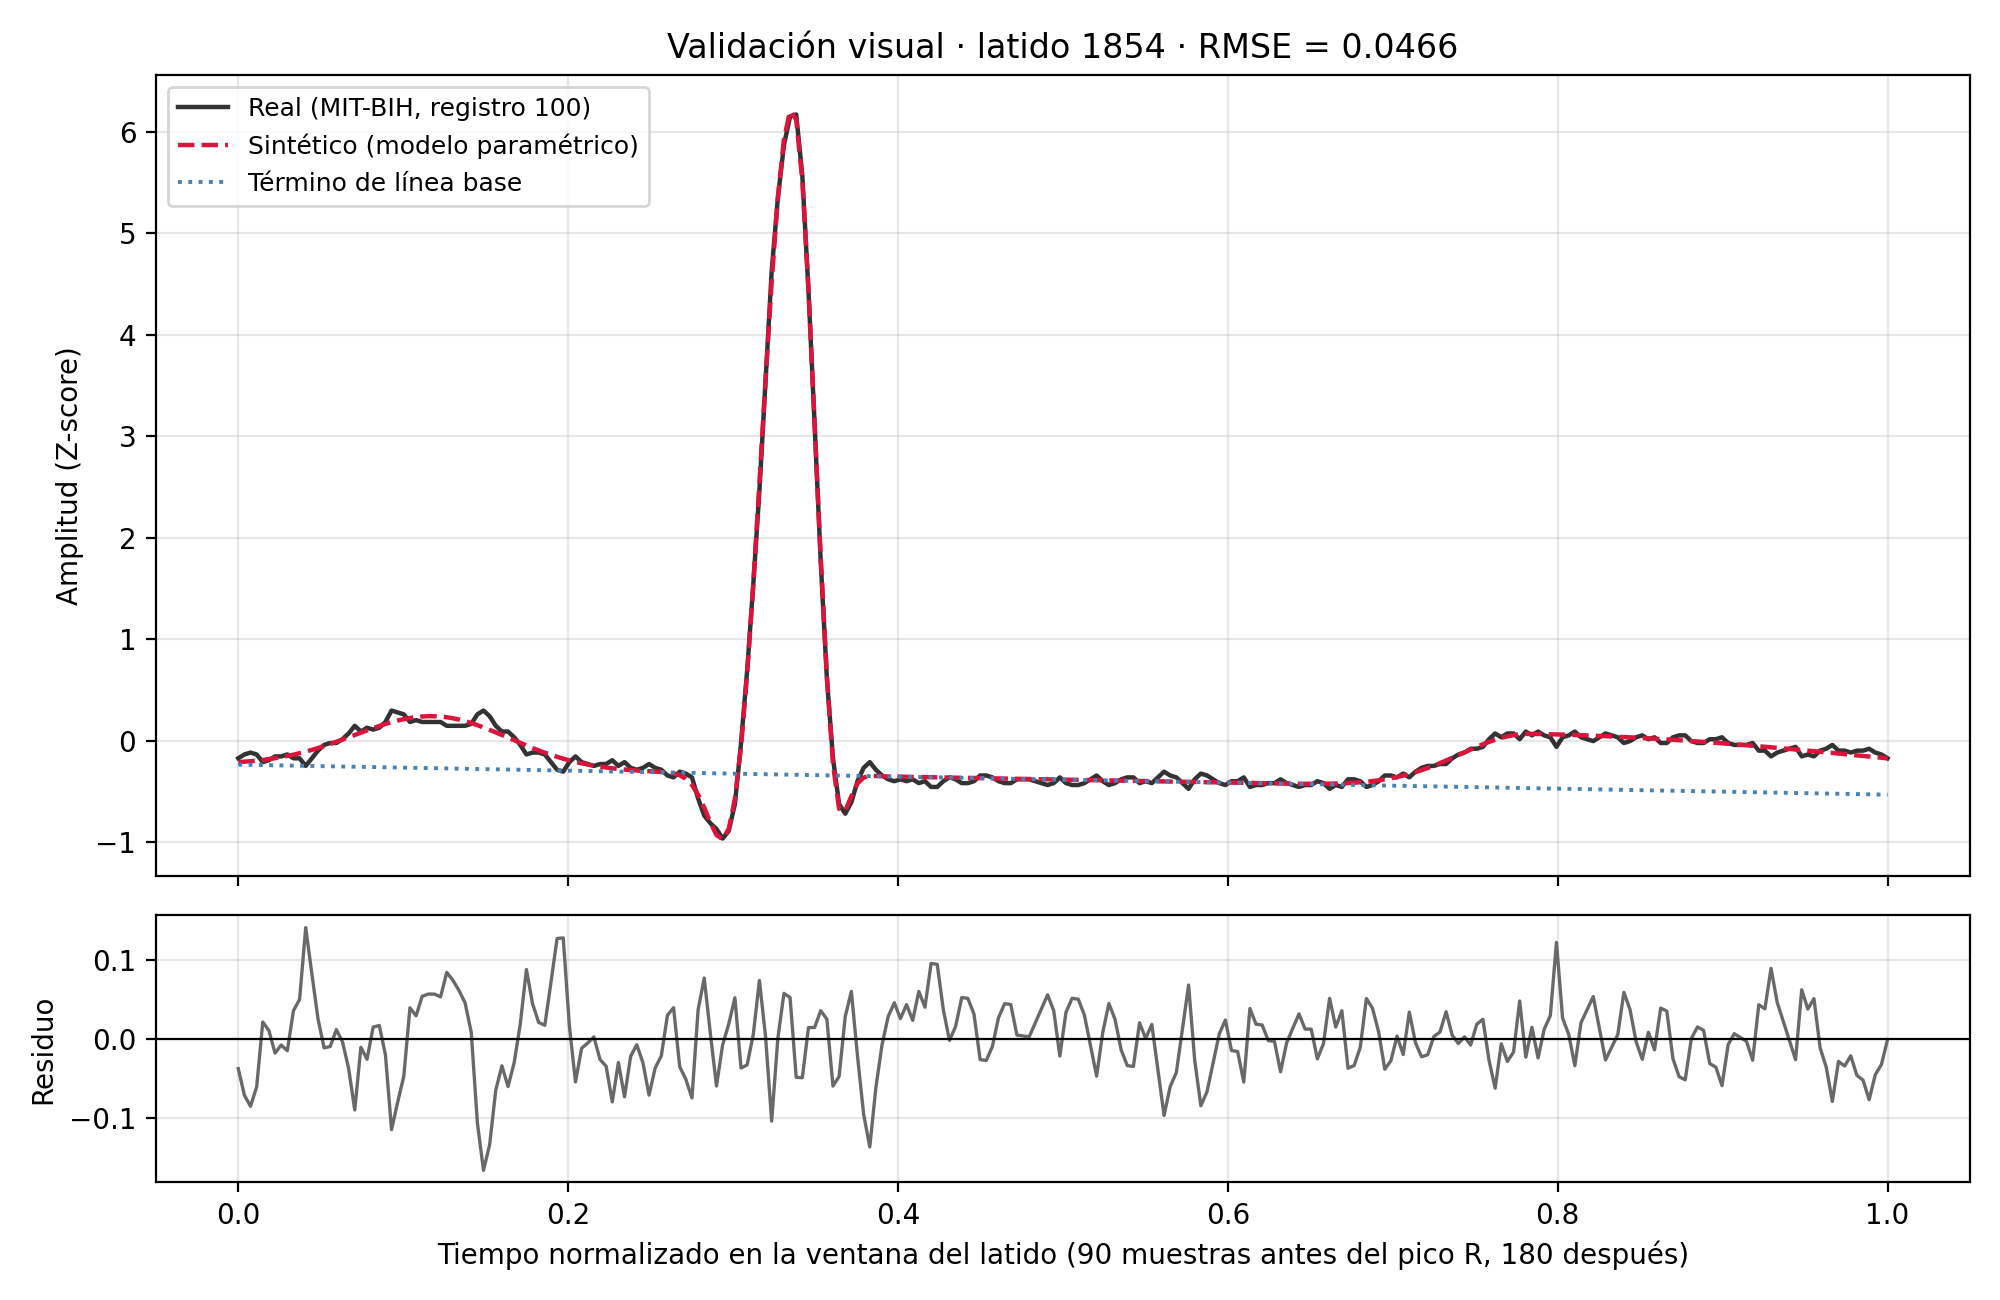
\includegraphics[width=0.95\textwidth]{fig/validacion_visual_v2.png}
\caption{Latido de mejor ajuste del registro 100 bajo la ventana asimétrica de 750 ms: latido 1854, con un RMSE de 0,0466, el mínimo del Cuadro \ref{tab:metricas}. La línea continua es el latido real, la discontinua el modelo ajustado, la punteada el término de línea base, y el panel inferior el residuo punto a punto. Los centros de las cinco ondas quedan dentro de la ventana; la rama descendente de la onda T, en cambio, no alcanza a volver a la línea base antes del borde derecho, que es la limitación que se discute en la Subsección \ref{sec:validez}.}
\label{fig:validacion}
\end{figure}

\subsection{Análisis del error residual y corrección del modelo}\label{sec:residuo}

La primera iteración del modelo, de veinte parámetros, alcanzó una correlación de Pearson media de 0,9647 y un RMSE medio de 0,3984. La lectura conjunta de ambas métricas exigía cautela: esa combinación no describe una reconstrucción de alta fidelidad en sentido estricto, sino un modelo que reproduce correctamente la \emph{forma} del ciclo P-QRS-T conservando una discrepancia de amplitud cercana a 0,4 desviaciones estándar de la señal normalizada. La correlación de Pearson es invariante ante transformaciones afines, de modo que un desplazamiento o un cambio de escala sistemáticos no la penalizan, mientras que sí penalizan el RMSE. Reportar únicamente la correlación habría sobreestimado el desempeño del generador.

El diagnóstico se apoyó en dos instrumentos distintos de la métrica agregada: el conteo de parámetros que convergen exactamente sobre un borde de su restricción de caja, y el sesgo medio del residuo. Un parámetro saturado indica que su valor quedó determinado por el límite y no por los datos; un sesgo no nulo indica una componente del error que el modelo no puede representar por construcción. Ambos instrumentos señalaron una causa concreta.

En primer lugar, se detectó una saturación sistemática en el límite superior del parámetro de amplitud de la onda R. Dicho límite estaba fijado en 3,5 unidades, y 2.234 de los 2.238 latidos (99,8\%) convergieron exactamente sobre esa cota. La causa de fondo es una inconsistencia de unidades: los límites de amplitud fueron derivados de rangos fisiológicos expresados en milivoltios, mientras que los latidos ingresan al ajuste normalizados por puntuación Z, donde el pico R del registro 100 alcanza 5,24 unidades. La restricción de caja, concebida para evitar artefactos, impedía reconstruir la deflexión de mayor amplitud del complejo.

La revisión completa del conteo de saturación mostró que el problema excedía a la onda R. En promedio, 11,8 de los 20 parámetros de cada latido quedaban fijados por un límite, y tres de ellos —el ancho ascendente de Q, el ancho descendente de S y el ancho descendente de T— saturaban en el 100\% de los latidos. El modelo no estaba siendo ajustado a los datos en más de la mitad de sus grados de libertad.

En segundo lugar, se verificó un sesgo sistemático entre ambas señales. El residuo medio, señal sintética menos real, fue de $+0{,}1457$ unidades normalizadas, atribuible a que el modelo de cinco Gaussianas carece de un término de línea base y retorna necesariamente a cero fuera de las deflexiones, mientras que la señal real presenta un desnivel en el segmento ST. Corregir por separado ese desplazamiento constante habría reducido el RMSE medio de 0,3984 a 0,3696, esto es, un 7,2\% del error total, lo que permitía concluir que el sesgo de línea base contribuía sin ser la causa principal del residuo. Esa conclusión resultó correcta: la causa principal era la inconsistencia de unidades en las restricciones de amplitud.

Se aplicaron ambas correcciones. El término de línea base se incorporó como dos parámetros adicionales del modelo, en lugar de restarse a posteriori, de modo que el optimizador lo ajusta simultáneamente con la morfología. Las restricciones de amplitud pasaron a expresarse como fracción del pico del latido. El Cuadro \ref{tab:ablacion} desagrega el aporte de cada corrección.

\begin{table}[H]
\centering
\begin{tabular}{|p{7.6cm}|c|c|}
\hline
\textbf{Configuración del modelo} & \textbf{Pearson} & \textbf{RMSE} \\ \hline
Primera iteración: 20 parámetros, restricciones en unidades de señal cruda & 0,9647 & 0,3984 \\ \hline
Se incorpora el término de línea base (22 parámetros) & 0,9763 & 0,3052 \\ \hline
Se corrigen las restricciones de amplitud, sin línea base (20 parámetros) & 0,9809 & 0,2285 \\ \hline
Ambas correcciones (22 parámetros) & 0,9986 & 0,0496 \\ \hline
\end{tabular}
\caption{Aporte de cada corrección, medido sobre los 2.238 latidos del registro 100. Cada fila corresponde a una corrida completa e independiente del ajuste, reproducible seleccionando el conjunto de restricciones y la presencia del término de línea base por línea de comandos.}
\label{tab:ablacion}
\end{table}

Cada corrección, por separado, mejora el error de forma modesta: la línea base lo reduce un 23,4\% y las restricciones corregidas un 42,7\%. Aplicadas juntas lo reducen un 87,6\%. El efecto conjunto no es, por lo tanto, la suma de los efectos individuales, y la razón es identificable. Mientras la amplitud de la onda R permanece fijada por su límite, el término de línea base absorbe parte del error de amplitud que corresponde a esa onda; y mientras no existe término de línea base, la amplitud liberada de R debe compensar el desnivel del segmento ST. Cada corrección despliega su efecto solo cuando la otra está presente, lo que explica que ninguna de las dos, por separado, anticipara la magnitud de la mejora conjunta.

Tras ambas correcciones el sesgo del residuo es nulo dentro de la precisión de la medición y el promedio de parámetros fijados por un límite cae de 11,8 de 20 a 1,8 de 22.

\subsection{Efecto de la redefinición de la ventana}
\label{sec:validez}

La limitación identificada en la iteración anterior era el largo de la ventana, y su corrección constituye el resultado más claro de esta etapa. Con la ventana centrada de 356 ms, el pico de la onda T caía fuera del recorte en 1.637 de los 2.238 latidos, con una posición mediana 98 ms más allá del borde, y la onda P ajustada presentaba una razón mediana de 7,63 entre sus anchos de subida y de bajada, con un máximo de 30. Una onda que sube siete veces más lento de lo que baja no es una onda P: es el resultado de ajustar una gaussiana contra un flanco parcial. Los parámetros de P y T de esa iteración eran, en consecuencia, artefactos del recorte y no descripciones morfológicas.

Con la ventana asimétrica de 750 ms, las cinco ondas caen dentro del recorte en los 2.237 latidos, y los centros ajustados medianos resultan $-159$ ms para P, $-24$ ms para Q, $+2$ ms para R, $+14$ ms para S y $+339$ ms para T, valores compatibles con la descripción clínica del complejo. La asimetría mediana del ancho de la onda P desciende de 7,63 a 1,23, y el promedio de parámetros determinados por una cota cae de 11,8 de 20 a 0,83 de 22.

\begin{figure}[H]
\centering
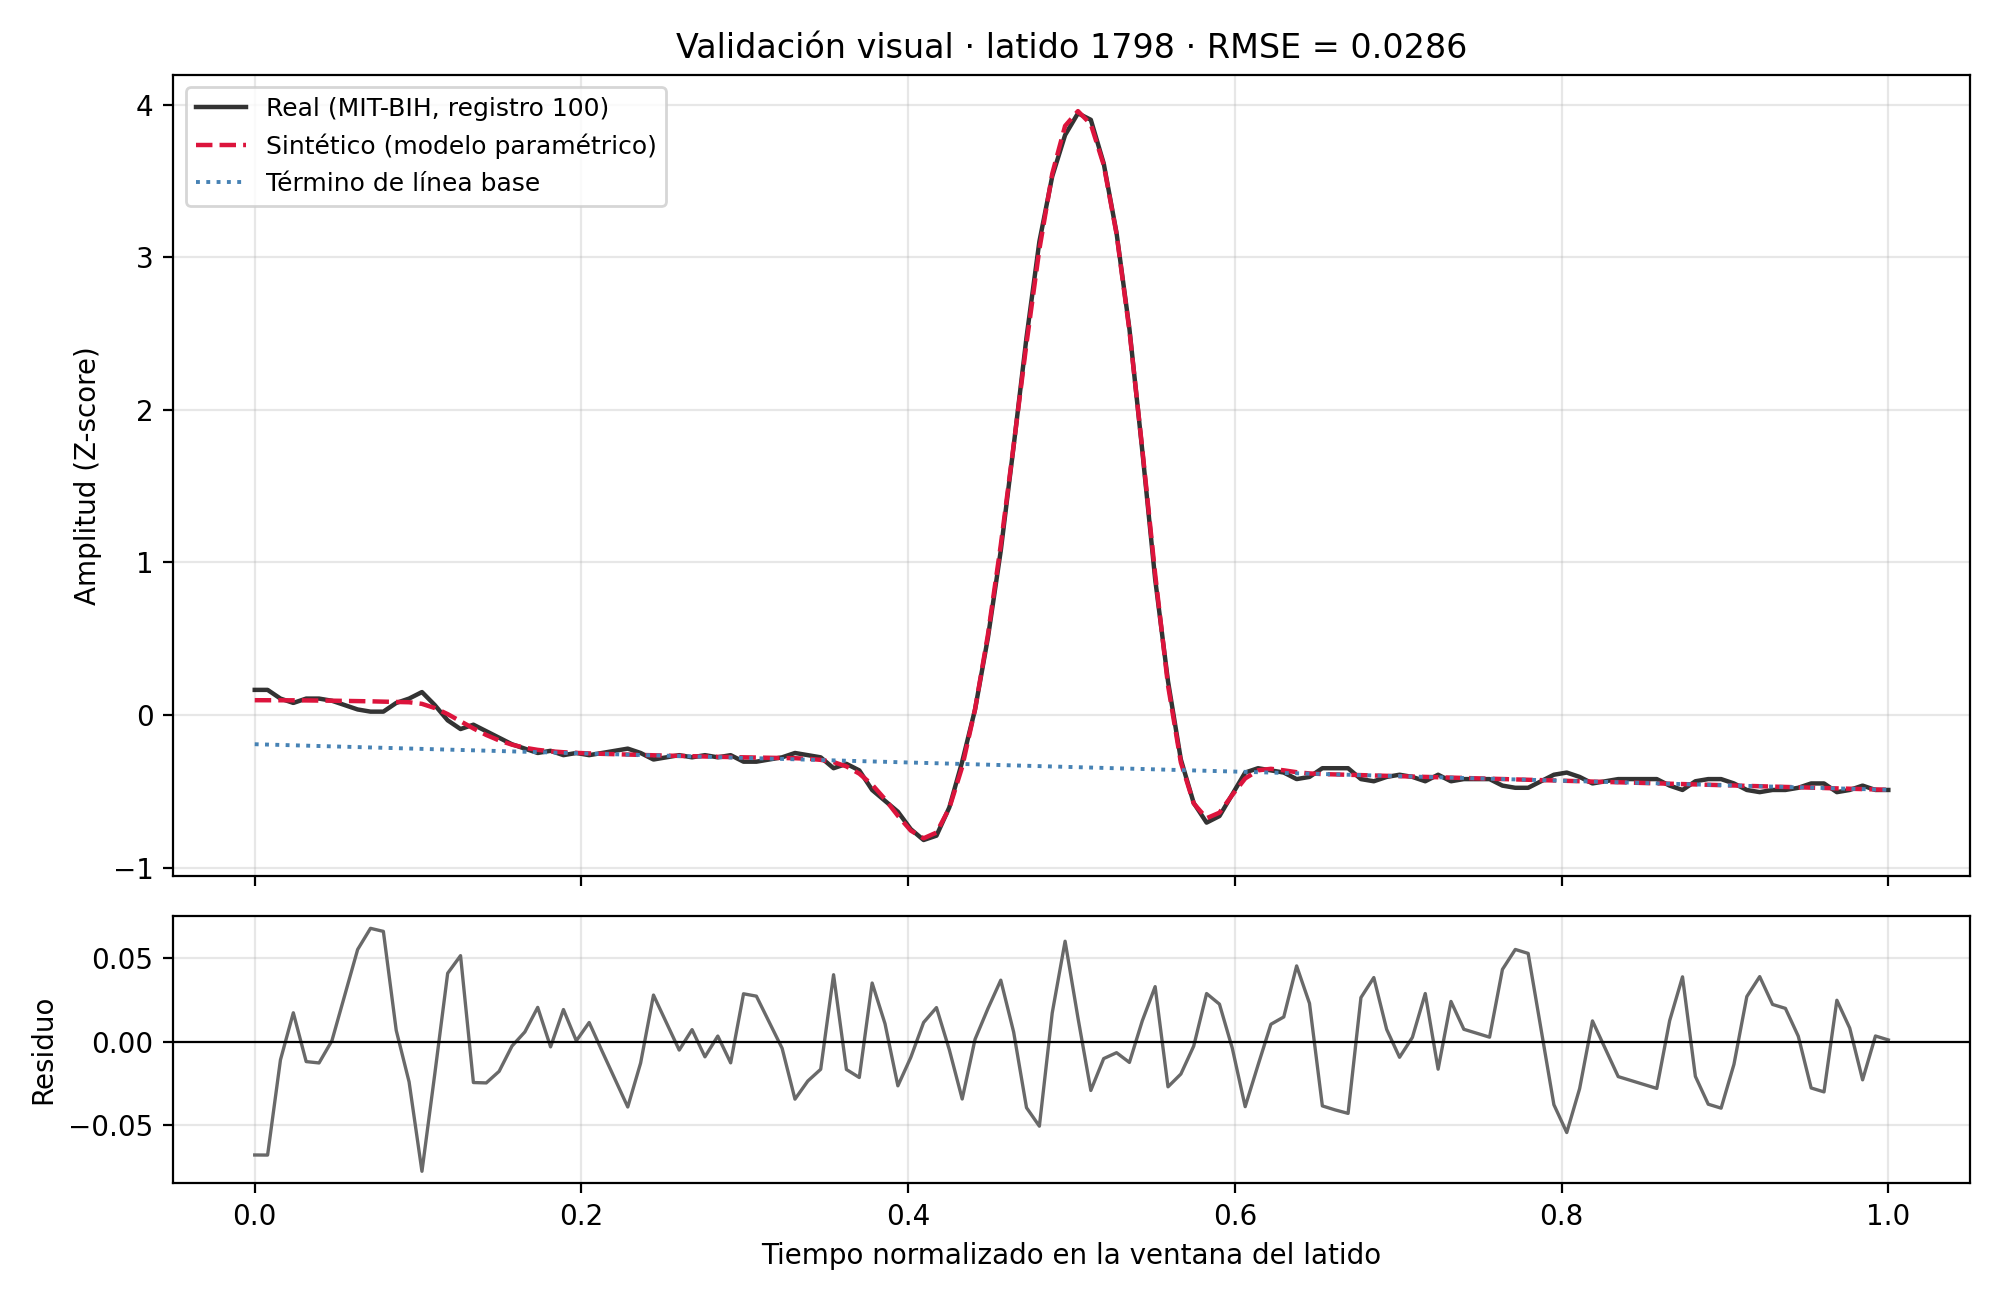
\includegraphics[width=0.85\textwidth]{fig/validacion_visual.png}
\caption{Latido de mejor ajuste de la segunda iteración, con la ventana centrada de 356 ms: latido 1798, RMSE de 0,0286. El recorte deja fuera el inicio de la onda P por la izquierda y la onda T por la derecha, de modo que el modelo ajusta sus gaussianas contra flancos incompletos. Su RMSE no es comparable con el de la Figura \ref{fig:validacion}, porque la ventana contiene menos de la mitad de la señal. Compárese con la Figura \ref{fig:validacion}, que muestra el mismo registro bajo la ventana asimétrica.}
\label{fig:validacion_v2}
\end{figure}

\subsubsection{Limitación remanente: la forma de la onda T}

La saturación no desaparece por completo. Un parámetro concentra prácticamente toda la que queda: el ancho de la rama descendente de la onda T converge sobre su cota de 180 ms en el 71,9\% de los latidos.

Se puso a prueba la hipótesis de que esa gaussiana estaba absorbiendo una deriva que la línea base afín no podía seguir a lo largo de 750 ms, agregando un término cuadrático de línea base como parámetro veintitrés, con el gradiente analítico extendido y verificado contra diferencias finitas. La hipótesis queda \emph{rechazada}: el RMSE mejora apenas un 2,3\%, de 0,0781 a 0,0763, y la saturación cae solo de 25 a 22 latidos de 40. Aflojar la cota produce un resultado análogo: con un tope de 300 ms el ajuste elige 232 ms y el error mejora un 2,7\%, y con un tope de 600 ms elige el mismo valor, de modo que es el dato y no la cota quien lo fija. Pero un ancho de 232 ms no describe una onda T, cuya duración total ronda los 160 ms: describe una deriva.

Se puso a prueba también la opción de representar la onda T con \emph{dos} gaussianas en lugar de una, llevando el modelo a veintiséis parámetros, con los centros ordenados por rango para que las dos componentes no fuesen intercambiables y con el gradiente analítico correspondiente verificado. Sobre cuarenta latidos, el RMSE mejora un 6,8\%, de 0,0776 a 0,0724, y el criterio de información bayesiano, que penaliza el número de parámetros, favorece al modelo de veintiséis por 15,4 unidades, una diferencia que se considera decisiva. Por ajuste, la segunda gaussiana se justifica. Pero la saturación, que era el problema a resolver, \emph{aumenta}: el promedio de parámetros determinados por una cota sube de 0,68 a 1,50 por latido, y la rama descendente de la última gaussiana de T pasa de saturar en 26 a saturar en 33 latidos de 40. El modelo de veintiséis parámetros ajusta mejor la señal, pero lo consigue con más parámetros cuyo valor fija el borde del dominio y no los datos, que es precisamente la condición que el control de saturación de la Sección \ref{sec:mp} declara invalidante para la interpretación fisiológica de un parámetro.

Ninguna de las tres hipótesis puestas a prueba —el término cuadrático de línea base, el aflojamiento de la cota y la segunda gaussiana— resuelve la saturación de la rama descendente de la onda T: las dos primeras apenas mejoran el error, y la tercera lo mejora a costa de aumentarla. La conclusión que sostiene la evidencia es, por lo tanto, más acotada que un rechazo: dentro de esta familia de funciones, la mejora de ajuste disponible se obtiene sacrificando la interpretabilidad de los parámetros, que es la propiedad que justifica un modelo paramétrico frente a uno de caja negra. Este trabajo conserva el modelo de veintidós parámetros por esa razón, y no porque el de veintiséis ajuste peor. La explicación remanente, visible en la Figura \ref{fig:validacion}, es que la onda T de este registro presenta una meseta ancha y no una campana, y una suma de gaussianas asimétricas no representa un plateau con parsimonia. La limitación se declara como tal, ahora acotada por medición y no por conjetura: corresponde explorar otra familia de funciones para la repolarización, y no ampliar la actual.

Vale registrar un detalle metodológico de esa prueba. Un primer intento, realizado sin gradiente analítico, produjo un RMSE \emph{peor} con \emph{más} parámetros, lo cual es imposible en un modelo anidado y por lo tanto delataba falta de convergencia y no una propiedad del modelo. Sin ese chequeo de coherencia se habría concluido lo contrario de lo correcto.

\subsection{Módulo de ritmo: recuperación del exponente prescrito}

Las secciones anteriores evalúan la forma del latido. Esta evalúa el tiempo
entre latidos, que es el aporte de esta versión del trabajo, y lo hace con un
criterio distinto: en lugar de preguntar si la serie generada se parece a una
real, se pregunta si posee la propiedad que se le pidió.

\subsubsection{Verificación del generador contra su propio estimador}

El primer control consiste en comprobar que la relación
$\alpha = (\beta+1)/2$ se cumple en la implementación. Sobre series de 32.768
puntos y doscientas realizaciones independientes por valor, el sesgo del
exponente recuperado no supera 0,011 en valor absoluto para $\alpha$ entre 0,6
y 1,4. Esto verifica el par generador-estimador de manera conjunta: un error en
cualquiera de los dos aparecería como una discrepancia sistemática mayor.

\subsubsection{Sesgo del estimador según el largo del registro}

El Cuadro \ref{tab:sesgo} reporta el exponente recuperado en función del
exponente pedido y del largo de la serie. Este cuadro no es un accesorio: es la
condición para poder interpretar un exponente medido sobre datos reales. El
sesgo es negativo, tiende a crecer con $\alpha$ y decrece con el largo del
registro, de modo que sin caracterizarlo no hay forma de distinguir un
exponente fisiológico de un artefacto de un registro corto.

\begin{table}[H]
\centering
\begin{tabular}{|c|c|c|c|}
\hline
\textbf{$\alpha$ pedido} & \textbf{$N=512$} & \textbf{$N=4.096$} & \textbf{$N=32.768$} \\ \hline
0,6 & $0{,}592 \pm 0{,}073$ & $0{,}593 \pm 0{,}030$ & $0{,}597 \pm 0{,}018$ \\ \hline
0,8 & $0{,}785 \pm 0{,}079$ & $0{,}792 \pm 0{,}037$ & $0{,}794 \pm 0{,}021$ \\ \hline
1,0 & $0{,}974 \pm 0{,}093$ & $0{,}986 \pm 0{,}040$ & $0{,}995 \pm 0{,}020$ \\ \hline
1,2 & $1{,}174 \pm 0{,}104$ & $1{,}184 \pm 0{,}044$ & $1{,}189 \pm 0{,}027$ \\ \hline
1,4 & $1{,}366 \pm 0{,}105$ & $1{,}383 \pm 0{,}048$ & $1{,}391 \pm 0{,}028$ \\ \hline
\end{tabular}
\caption{Exponente recuperado de la serie generada, como media $\pm$ desviación estándar sobre doscientas realizaciones independientes por celda; el error estándar del sesgo no supera 0,008. El sesgo del estimador es negativo, tiende a crecer con el exponente y decrece con el largo del registro.}
\label{tab:sesgo}
\end{table}

\subsubsection{Cohorte sintética de veinticuatro horas}

Se generó una cohorte de cincuenta sujetos sintéticos de veinticuatro horas cada
uno, con 101.647 latidos por sujeto y un exponente sorteado por sujeto de una
distribución normal, de modo que la cohorte tenga dispersión entre individuos y
no un único exponente repetido. La correlación entre el exponente pedido y el
recuperado es de 0,98, con un error absoluto medio de 0,014, y ningún intervalo
requirió recorte por salirse del rango fisiológico. El exponente de corto
alcance de la cohorte resultó $\alpha_1 = 1{,}17 \pm 0{,}09$, unas tres
centésimas por encima del exponente global recuperado, $1{,}14$. Esa diferencia
no debe leerse como un cruce de pendiente: el generador es monofractal, produce
un único exponente en todas las escalas, y el exceso de $\alpha_1$ es
consistente con el sesgo positivo del estimador en ventanas de pocos latidos
descrito en la Sección \ref{sec:mp}. Tampoco debe leerse como una validación
frente al valor de 1,17 reportado para adultos sanos
\cite{costa2017fragmentation}: el exponente que se le pidió a la cohorte se
sorteó de una distribución centrada precisamente en ese valor. Reproducir el
cruce entre $\alpha_1$ y $\alpha_2$ que se observa en sujetos sanos exigiría
un generador con dos regímenes de escalamiento, y queda planteado como
extensión.

\begin{figure}[H]
\centering
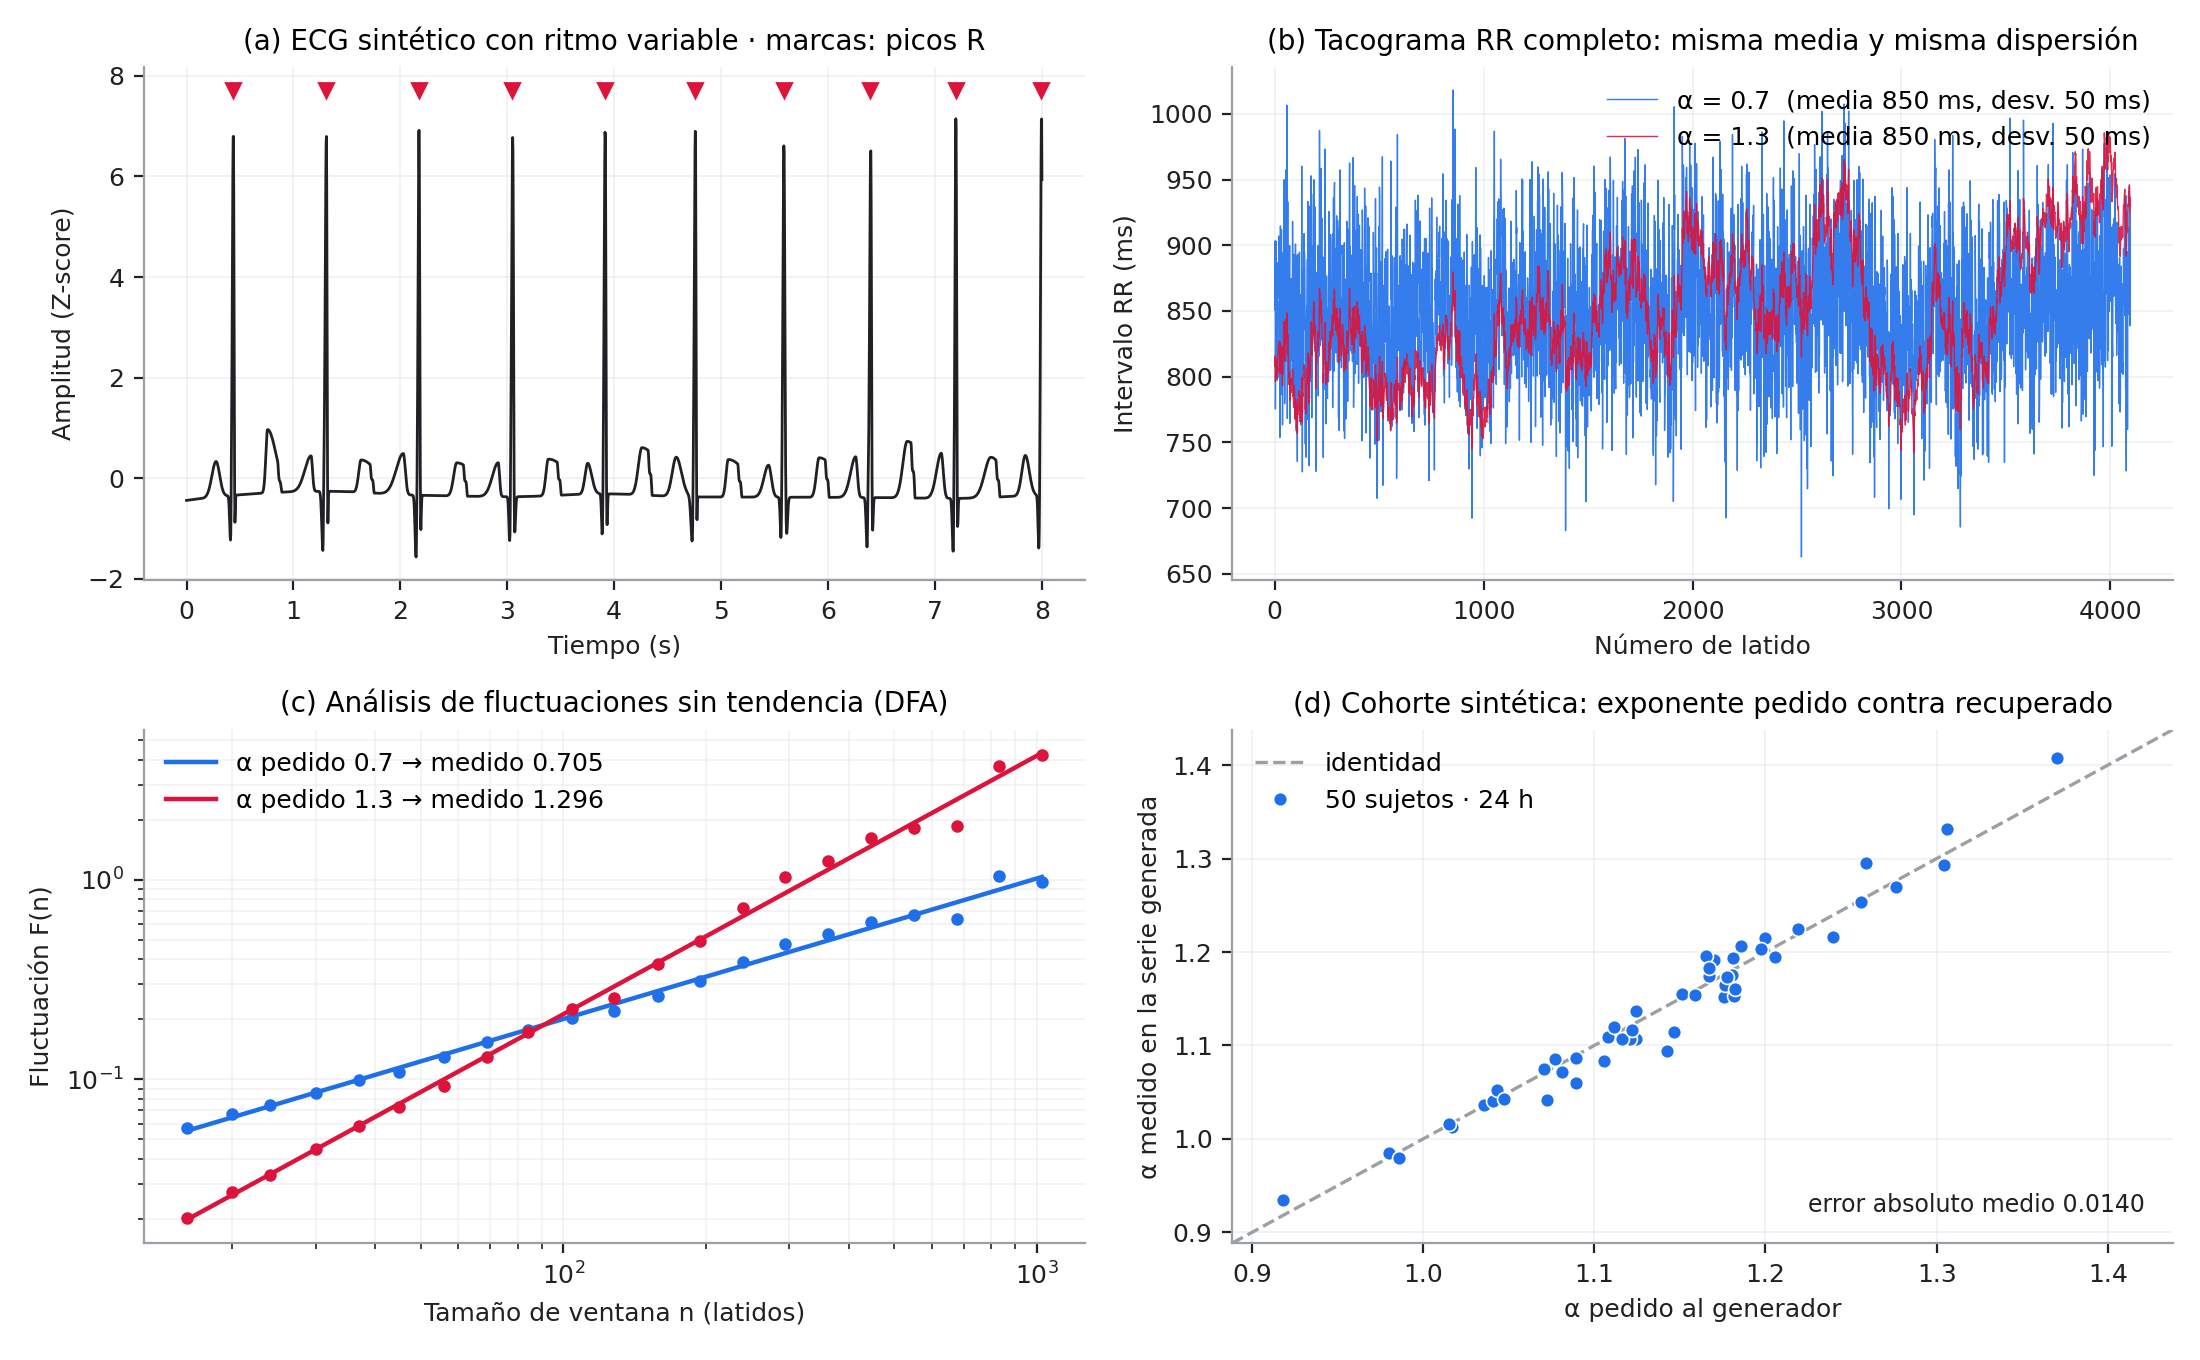
\includegraphics[width=\textwidth]{fig/validacion_hurst.png}
\caption{Validación del módulo de ritmo. (a) Ocho segundos de ECG sintético con ritmo variable; las marcas señalan los picos R. (b) Dos tacogramas R-R con la misma media y la misma desviación estándar pero distinto exponente de escalamiento. (c) Análisis de fluctuaciones sin tendencia de esas dos series, con el exponente pedido y el recuperado. (d) Cohorte de cincuenta sujetos sintéticos de veinticuatro horas: exponente pedido contra exponente recuperado, con la recta identidad como referencia.}
\label{fig:ritmo}
\end{figure}

El panel (b) de la Figura \ref{fig:ritmo} muestra el punto de toda la
construcción. Los dos tacogramas comparten media y desviación estándar, de modo
que cualquier índice convencional de variabilidad en el dominio del tiempo los
reportaría como equivalentes; difieren únicamente en la organización temporal de
sus fluctuaciones, que es la dimensión que el exponente captura y que esos
índices no ven.

\subsection{Motor de reglas fisiológicas: cohorte etiquetada}\label{sec:cohorte}

Se generó una cohorte de 500 sujetos sanos y 500 enfermos con el motor descrito en la Subsección~\ref{sec:reglas}, con semilla 0, sobre la plantilla morfológica de los 2.237 latidos ajustados y en el estrato de referencia de hombres de 60 a 69 años. El archivo de la cohorte registra la semilla, el estrato, el conjunto de parámetros de origen, la geometría de la ventana y el entorno de cálculo, de modo que puede regenerarse exactamente.

El Cuadro~\ref{tab:cohorte} resume la verificación. Ninguna de las cinco condiciones falla en ninguno de los mil sujetos.

\begin{table}[H]
\centering
\begin{tabular}{|p{9cm}|c|}
\hline
\textbf{Condición verificada} & \textbf{Sujetos que la incumplen} \\ \hline
Rasgo impuesto con error mayor a 1 ms & 0 de 1.000 \\ \hline
Sujeto sano con un rasgo impuesto fuera de su rango & 0 de 500 \\ \hline
Sujeto enfermo con su rasgo desviado dentro del rango & 0 de 500 \\ \hline
Onda T solapada con el complejo QRS & 0 de 1.000 \\ \hline
Centro de la onda T fuera de la ventana de extracción & 0 de 1.000 \\ \hline
\end{tabular}
\caption{Verificación de la cohorte de 500 sujetos sanos y 500 enfermos, medida sobre los parámetros efectivamente generados.}
\label{tab:cohorte}
\end{table}

En el grupo de enfermos, el rasgo desviado se distribuyó entre 131 sujetos por el intervalo PR, 132 por la duración del QRS, 130 por el intervalo QT y 107 por la duración de la onda P. En el grupo control, los intervalos medidos cubren los rangos de referencia completos: el PR va de 114,0 a 216,0~ms, el QRS de 76,0 a 113,9~ms y el QT de 338,6 a 471,5~ms. Este último alcanza valores por encima de 450~ms sin que ello constituya un error de etiquetado, por las razones expuestas en la Subsección~\ref{sec:reglas}: se trata de QT sin corregir por frecuencia. El centro de la onda T de los sujetos sanos se ubica entre 122 y 316~ms después del pico R; en ausencia de un rango de referencia para esa posición, la cifra se informa como observación y no como criterio de validez.

\subsection{Alcance efectivo respecto a los resultados proyectados}

Por transparencia metodológica, el Cuadro \ref{tab:alcance} contrasta los resultados proyectados en la propuesta de esta investigación con lo efectivamente alcanzado hasta la fecha.

\begin{table}[H]
\centering
\begin{tabular}{|p{7cm}|p{6.5cm}|}
\hline
\textbf{Resultado proyectado} & \textbf{Estado actual} \\ \hline
Framework de generación paramétrica en Python & Implementado y funcional para latidos sinusales normales \\ \hline
Validación de fidelidad frente a MIT-BIH & Realizada sobre 1 registro de los 48 de la base \\ \hline
Dataset de al menos 5.000 latidos sintéticos & 2.237 latidos parametrizados, más una cohorte de 50 series de 24 horas \\ \hline
Motor de reglas fisiológicas para grupo control y grupo de enfermos & Implementado y verificado sobre una cohorte de 500 sanos y 500 enfermos, en un estrato de referencia fijo \\ \hline
Validación del conjunto sintético con red neuronal preentrenada & No realizada \\ \hline
Publicación en revista indexada & Pendiente \\ \hline
\end{tabular}
\caption{Contraste entre los resultados proyectados y los alcanzados.}
\label{tab:alcance}
\end{table}

El motor de reglas fisiológicas se implementó y verificó con dos restricciones de alcance: opera sobre un único estrato de referencia, sin variar el sexo ni la edad, y construye sus etiquetas solo sobre intervalos morfológicos, sin intervención del exponente de escalamiento del ritmo. La validación del conjunto sintético mediante un modelo preentrenado queda fuera del alcance de esta etapa. En consecuencia, las conclusiones sobre fidelidad morfológica son válidas para ritmo sinusal normal, y las etiquetas del motor describen cómo se construyó cada sujeto, no una condición clínica.

\subsection{Resultados de responsabilidad social}

El proyecto pretende democratizar el acceso a datos médicos de alta calidad sin comprometer la privacidad de los pacientes. Al proporcionar un generador robusto, se facilita que investigadores en regiones con pocos recursos clínicos puedan desarrollar y validar sus propios algoritmos de diagnóstico cardiovascular, promoviendo la equidad en las tecnologías de salud asistida.

\end{spacing}

\newpage
\section{Conclusiones y trabajos futuros}
\begin{spacing}{1.5}

\subsection{Conclusiones}
\label{sec:conclusiones}

A partir de los resultados obtenidos se extraen las siguientes conclusiones, organizadas según el grado de cumplimiento de los objetivos específicos planteados.

\subsubsection{Sobre los objetivos alcanzados}

\begin{itemize}
    \item \textbf{Viabilidad del modelado paramétrico (objetivo 1).} La superposición de cinco funciones Gaussianas asimétricas, complementada con un término de línea base, reproduce la morfología del ciclo P-QRS-T en ritmo sinusal normal con una correlación de Pearson media de 0,9986 y un RMSE medio de 0,0496 sobre 2.238 latidos. Las desviaciones estándar respectivas, 0,0020 y 0,0162, indican que el desempeño es estable a lo largo del registro y no depende de latidos favorables aislados.

    \item \textbf{Eficacia de la optimización con restricciones (objetivo 2).} El algoritmo L-BFGS-B \cite{byrd1995limited} con restricciones de caja permitió ajustar los veintidós parámetros del modelo a cada latido individual sin generar morfologías biológicamente imposibles. El resultado depende, no obstante, de que las restricciones estén expresadas en las mismas unidades que la señal a la que se aplican. La primera implementación derivó sus cotas de amplitud de rangos fisiológicos en milivoltios y las aplicó a latidos normalizados por puntuación Z: el 99,8\% de los latidos convergió exactamente sobre la cota superior de la amplitud de la onda R y, en promedio, 11,8 de los 20 parámetros quedaron determinados por un límite en lugar de por los datos. Expresadas las cotas de amplitud como fracción del pico de cada latido, ese promedio desciende a 1,8 de 22.

    \item \textbf{Valor diagnóstico del residuo frente a la métrica agregada.} La correlación de Pearson de la primera iteración, 0,9647, era compatible con un modelo cuya mayoría de parámetros no estaba siendo ajustada por los datos. Fueron dos indicadores auxiliares —el conteo de parámetros saturados en sus cotas y el sesgo medio del residuo— los que localizaron ambos defectos y guiaron una corrección que redujo el RMSE en un 87,6\%. Reportar métricas agregadas de fidelidad sin instrumentar el residuo habría dejado ese margen sin detectar.

    \item \textbf{Interpretabilidad frente a los modelos generativos profundos.} Cada parámetro del modelo posee un significado fisiológico directo, propiedad de la que carecen las arquitecturas basadas en redes generativas antagónicas \cite{brophy2023generative}. Esta característica es una ventaja estructural del enfoque, si bien su valor práctico para la aumentación de datos requiere validación adicional.
\end{itemize}

\subsubsection{Sobre los objetivos no alcanzados}

La honestidad metodológica exige declarar que tres de los cinco objetivos específicos no fueron completados en esta etapa:

\begin{itemize}
    \item El motor de reglas fisiológicas basado en las tablas de Rijnbeek \cite{rijnbeek2001normal} y de la AHA \cite{rautaharju2009aha} (objetivo 3) no fue implementado. En consecuencia, el generador no produce, por ahora, variabilidad demográfica por edad ni por sexo.

    \item El modelado de alteraciones patológicas (objetivo 4), específicamente la elevación del segmento ST y la Fibrilación Auricular, tampoco fue abordado.

    \item La validación (objetivo 5) se completó parcialmente: se calcularon la correlación de Pearson y el RMSE, pero no se realizó el análisis en el dominio de la frecuencia comprometido en la propuesta.
\end{itemize}

\subsubsection{Sobre la hipótesis}

La hipótesis planteada sostenía que es posible construir un generador de señales ECG sintéticas basado en Gaussianas y optimización numérica que reproduzca la morfología de señales reales con alta fidelidad estructural, permitiendo además la parametrización controlada por edad, sexo y condición patológica.

La evidencia obtenida valida la primera parte de la hipótesis y deja la segunda sin verificar. La reproducción morfológica quedó demostrada para ritmo sinusal normal en población adulta. La parametrización demográfica y patológica no fue puesta a prueba, por lo que no puede afirmarse ni refutarse con los datos disponibles.

Corresponde asimismo precisar la expresión ``alta fidelidad''. La primera iteración del modelo alcanzaba una correlación de 0,9647 con un RMSE de 0,3985, combinación que describe una reconstrucción morfológicamente correcta pero con una discrepancia de amplitud apreciable: la correlación de Pearson es invariante ante transformaciones afines y, por sí sola, sobreestima el desempeño del generador. En el modelo corregido ambas métricas son consistentes entre sí —0,9986 y 0,0496— de modo que la expresión resulta defendible, si bien únicamente para ritmo sinusal normal en población adulta.

\subsection{Trabajos Futuros}

Las líneas de trabajo inmediatas se desprenden directamente de las limitaciones identificadas en la sección de resultados:

\begin{enumerate}
    \item \textbf{Redefinir la ventana de extracción.} La ventana de 128 muestras a 360 Hz cubre 356 ms, mientras que un complejo P-QRS-T normal se extiende entre 600 y 800 ms. Las ondas P y T quedan parcialmente fuera del recorte y sus anchos permanecen determinados por sus cotas en cerca de la mitad de los latidos, pese a la corrección de las restricciones. Ampliar la ventana obliga a redefinir la unidad de análisis y a recalcular las métricas reportadas, por lo que constituye una decisión metodológica y no un ajuste de implementación.

    \item \textbf{Extender la validación al conjunto de la base.} Los resultados presentados corresponden a un único registro de los 48 que componen MIT-BIH. La generalización del método exige repetir el procedimiento sobre el conjunto completo y reportar la variabilidad entre registros.

    \item \textbf{Implementar el motor de reglas demográficas.} Integrar las tablas de Rijnbeek \cite{rijnbeek2001normal} y de la AHA \cite{rautaharju2009aha} para modular los intervalos PR, QRS y QT según edad y sexo, y validar las señales resultantes contra rangos de referencia clínicos.

    \item \textbf{Modelar alteraciones patológicas.} Incorporar la elevación del segmento ST mediante funciones de lesión y la Fibrilación Auricular mediante estocasticidad del intervalo R-R con anulación de la onda P.

    \item \textbf{Completar la validación en el dominio de la frecuencia.} Contrastar los espectros de potencia de las señales sintéticas y reales, según lo comprometido en el quinto objetivo específico.

    \item \textbf{Validar la utilidad para aumentación de datos.} La justificación última de este trabajo es mejorar el entrenamiento de clasificadores de arritmias. Corresponde entrenar un clasificador con datos reales, repetir el entrenamiento incorporando las señales sintéticas y medir la diferencia de desempeño. Sin este experimento, la utilidad práctica del generador permanece como hipótesis.
\end{enumerate}

\end{spacing}

\newpage
%\section{Anexos}
\begin{spacing}{1.5}

\subsection{Cronograma original de la propuesta}

El plan de trabajo de esta investigación se estructuró en tres semestres académicos, alineando cada fase con los objetivos específicos planteados, desde la fundamentación teórica hasta la validación del modelo generativo.

A continuación, se detalla el cronograma perteneciente al primer semestre del año 2025, enfocado en el diseño base:

\begin{table}[H]
\centering
\renewcommand{\arraystretch}{1.3}
\begin{tabular}{|p{6.5cm}|c|c|c|c|c|c|}
\hline
\textbf{Actividad} & \textbf{Mar} & \textbf{Abr} & \textbf{May} & \textbf{Jun} & \textbf{Jul} & \textbf{Ago} \\ \hline
Revisión del Estado del Arte & X & X & & & & \\ \hline
Extracción y preprocesamiento MIT-BIH & & & X & X & & \\ \hline
Diseño del modelo matemático Gaussiano & & & & X & X & X \\ \hline
\end{tabular}
\caption{Cronograma de Actividades Primer Semestre 2025.}
\label{tab:crono1}
\end{table}

El cronograma perteneciente al segundo semestre del año 2025 contempla la implementación de los motores de optimización y reglas clínicas:

\begin{table}[H]
\centering
\renewcommand{\arraystretch}{1.3}
\begin{tabular}{|p{6.5cm}|c|c|c|c|c|c|}
\hline
\textbf{Actividad} & \textbf{Sep} & \textbf{Oct} & \textbf{Nov} & \textbf{Dic} & \textbf{Ene} & \textbf{Feb} \\ \hline
Implementación optimización L-BFGS-B & X & X & & & & \\ \hline
Motor de reglas demográficas & & X & X & X & & \\ \hline
Modelado de patologías (FA, IAM) & & & & & X & X \\ \hline
\end{tabular}
\caption{Cronograma de Actividades Segundo Semestre 2025.}
\label{tab:crono2}
\end{table}

Finalmente, el cronograma perteneciente al primer semestre del año 2026 se centra en la validación estadística y redacción final:

\begin{table}[H]
\centering
\renewcommand{\arraystretch}{1.3}
\begin{tabular}{|p{6.5cm}|c|c|c|c|c|c|}
\hline
\textbf{Actividad} & \textbf{Mar} & \textbf{Abr} & \textbf{May} & \textbf{Jun} & \textbf{Jul} & \textbf{Ago} \\ \hline
Pruebas de validación (RMSE, Pearson) & X & X & & & & \\ \hline
Análisis de resultados y métricas & & & X & & & \\ \hline
Escritura del documento de Tesis & & & X & X & X & \\ \hline
Entrega y Defensa de Tesis & & & & & & X \\ \hline
\end{tabular}
\caption{Cronograma de Actividades Primer Semestre 2026.}
\label{tab:crono3}
\end{table}

\end{spacing}
  
\newpage

%\newpage

% ----------------------------------------------------------------
%\newpage % Salto de pagina para poner referencias solas en una pagina
%\bibliographystyle{abbrv}
%\bibliography{BiblioRegistracion}
\newpage
\bibliographystyle{plain}
% https://www.overleaf.com/learn/latex/bibtex_bibliography_styles
%\bibliographystyle{APA/apa-good}
%\bibliographystyle{alpha}
\bibliography{biblio}
\pagestyle{fancy}

\end{document}

